\documentclass[UTF8]{ctexart}
\usepackage[table]{xcolor}
\usepackage{algorithm}
\usepackage{algorithmic}
\usepackage{subfigure}
\usepackage{amsmath,bm}
\usepackage{fancybox}
\usepackage{listings}
\usepackage{xcolor}
\usepackage{diagbox}
\usepackage{amssymb}
\usepackage{amsmath}
\usepackage{amsthm}
\usepackage{empheq}
\usepackage{warpcol}
\usepackage{lscape}
\usepackage[framemethod=tikz]{mdframed}
\usepackage{mathtools}
\usepackage{fancyhdr} 
\usepackage{longtable,booktabs}                               
\usepackage{lastpage}                                           
\usepackage{layout} 


% 图表
\usepackage{array,multirow}
  \setlength\extrarowheight{2pt} % 行高增加
\usepackage{longtable}
\usepackage{graphicx}

\usepackage{listings}

\usepackage{xcolor}

	\definecolor{ocre}{RGB}{243,102,25}
	\definecolor{mygray}{RGB}{243,243,244}

%
%\lstset{
%columns=flexible,
%numbers=left,
%numberstyle=\footnotesize\color{darkgray}, 
%basicstyle=\small\ttfamily,
%stringstyle=\color{purple},
%keywordstyle=\color[RGB]{40,40,255}\bfseries,
%commentstyle=\it\color[RGB]{0,96,96},  
%stringstyle=\rmfamily\slshape\color[RGB]{128,0,0}, 
%showstringspaces=false,      
%% directivestyle=\color{blue},
%frame=shadowbox,
%%framerule=0pt,
%backgroundcolor=\color[RGB]{245,245,244},
%escapeinside=``, %逃逸字符(1左面的键),用于显示中文
%breaklines,
%extendedchars=false,
%%解决代码跨页时,章节标题,页眉等汉字不显示的问题
%xleftmargin=2em,xrightmargin=2em,
%aboveskip=1em,%设置边距
%tabsize=4, %设置tab空格数  
%showspaces=false %不显示空格 
%rulesepcolor=\color{red!20!green!20!blue!20}
%%rulesepcolor=\color{brown}
%}



% 行号
\usepackage{lineno}


% 引用
\usepackage[colorlinks=true,
            pdfborder=001,     
            citecolor=blue,
            linkcolor=red,
            anchorcolor=green,
            urlcolor=blue,
            bookmarksopen=true,bookmarksnumbered=true]{hyperref}
\usepackage{framed} 
\usepackage{ulem}
\usepackage[numbered,framed]{matlab}
\begin{document}
\thispagestyle{empty}
	\begin{figure}[h]
		\centering
		
\includegraphics[width=5.5cm]{fig/logo.jpg}
	\end{figure}

	\vspace*{0.5cm}
	\begin{center}
		\Huge{\textbf{\heiti BP算法仿真实验}}
	\end{center}
	
	\vspace*{0.5cm}
	
	\begin{table}[h]
		\centering	
		\begin{Large}
			\begin{tabular}{p{3cm}<{\raggedleft} p{6cm}<{\centering}}
				\textbf{作\qquad 者:} & {\kaishu 张晋} \\
				%\cline{2-2}
				\textbf{学\qquad 号: }& 15091060 \\
				%\cline{2-2}
				\textbf{学\qquad 院:} & {\kaishu 数学与系统科学学院}\\
				%\cline{2-2}
				\textbf{学\qquad 校: }& {\kaishu 北京航空航天大学} \\
				%\cline{2-2}
				\textbf{指导教师:} & {\kaishu 刘红英}\\
				%\cline{2-2}
			\end{tabular}
		\end{Large}
	\end{table}
	


\vspace*{1cm}
	



\newpage
\tableofcontents
\newpage
\newpage
\section{BP算法}
\subsection{核心迭代公式}
\begin{center}
  \begin{minipage}{0.7\textwidth}
    \begin{framed}
      \centering
      \textbf{前向传播的三个方程式}\label{backpropsummary}\\
      \vspace{1.5ex}
      \begin{tabular}{ll}
        $\bm{z}^l=\bm{w}^l\bm{a}^{l-1}+\bm{b}^l$            & \hspace{2cm} \\[1.5ex]
        $\bm{a}^l=\sigma\left(\bm{w}^l\bm{a}^{l-1}+\bm{b}^l\right)=\sigma(\bm{z}^l)$ & \hspace{2cm} \\[1.5ex]
        $E=\text{Cost}(\bm{y},\bm{a}^L )$       & \hspace{2cm} \\[1.5ex]
      
      \end{tabular}
    \end{framed}
  \end{minipage}
\end{center}

我们记$\bm{\delta} ^l=\dfrac{\partial E}{\partial\bm{z}^l}$,则有:
\begin{center}
  \begin{minipage}{0.7\textwidth}
    \begin{framed}
      \centering
      \textbf{反向传播的四个方程式}\label{backpropsummary}\\
      \vspace{1.5ex}
      \begin{tabular}{ll}
        $\bm{\delta}^L = \dfrac{\partial E}{\partial\bm{a}^L}\odot\sigma'(\bm{z}^L)$            & \hspace{2cm} \\[1.5ex]
        $\bm{\delta}^l = ((\bm{w}^{l+1})^T \bm{\delta}^{l+1}) \odot \sigma'(\bm{z}^l)$ & \hspace{2cm} \\[1.5ex]
        $\dfrac{\partial E}{\partial \bm{b}^l} = \bm{\delta}^l$       & \hspace{2cm} \\[1.5ex]
        $\dfrac{\partial E}{\partial \bm{w}^l} = \bm{\delta}^l(\bm{a}^{l-1})^T$ & \hspace{2cm}
      \end{tabular}
    \end{framed}
  \end{minipage}
\end{center}







\newpage
\section{XOR异或问题}
\begin{table}[htbp]
  \centering
  \caption{XOR问题}
    \begin{tabular}{ccc}
    \toprule
    \multicolumn{2}{c}{\textbf{Input}} & \textbf{Output} \\
    \midrule
    0     & 0     & 0 \\

    \rowcolor[rgb]{0.973, 0.973, 0.973} 0     & 1     & 1 \\

    1     & 0     & 1 \\

    \rowcolor[rgb]{0.973, 0.973, 0.973} 1     & 1     & 0 \\
    \bottomrule
    \end{tabular}%
  \label{XOR}%
\end{table}%

\subsection{二次函数代价函数}
%\[\begin{array}{l}
%E = \frac{1}{m}\sum\limits_x {{{\left\| {{a_3} - y} \right\|}^2}} \\
%\frac{{\partial E}}{{\partial {a_3}}} = \frac{2}{m}\sum\limits_x {({a_3} - y)} \\
%{\delta _3} = \frac{{\partial E}}{{\partial {z_3}}} = \frac{2}{m}\sum\limits_x {({a_3} - y)}  \odot \sigma '({z_3})\\
%{\delta _2} = {w_3}^T{\delta _3} \odot \sigma '({z_2})\\
%\frac{{\partial E}}{{\partial {b_2}}} = {\delta _2}\\
%\frac{{\partial E}}{{\partial {w_2}}} = {\delta _2}{a_1}^T
%\end{array}\]
首先我们选用二次函数作为代价函数
\begin{figure}[H]
\centering
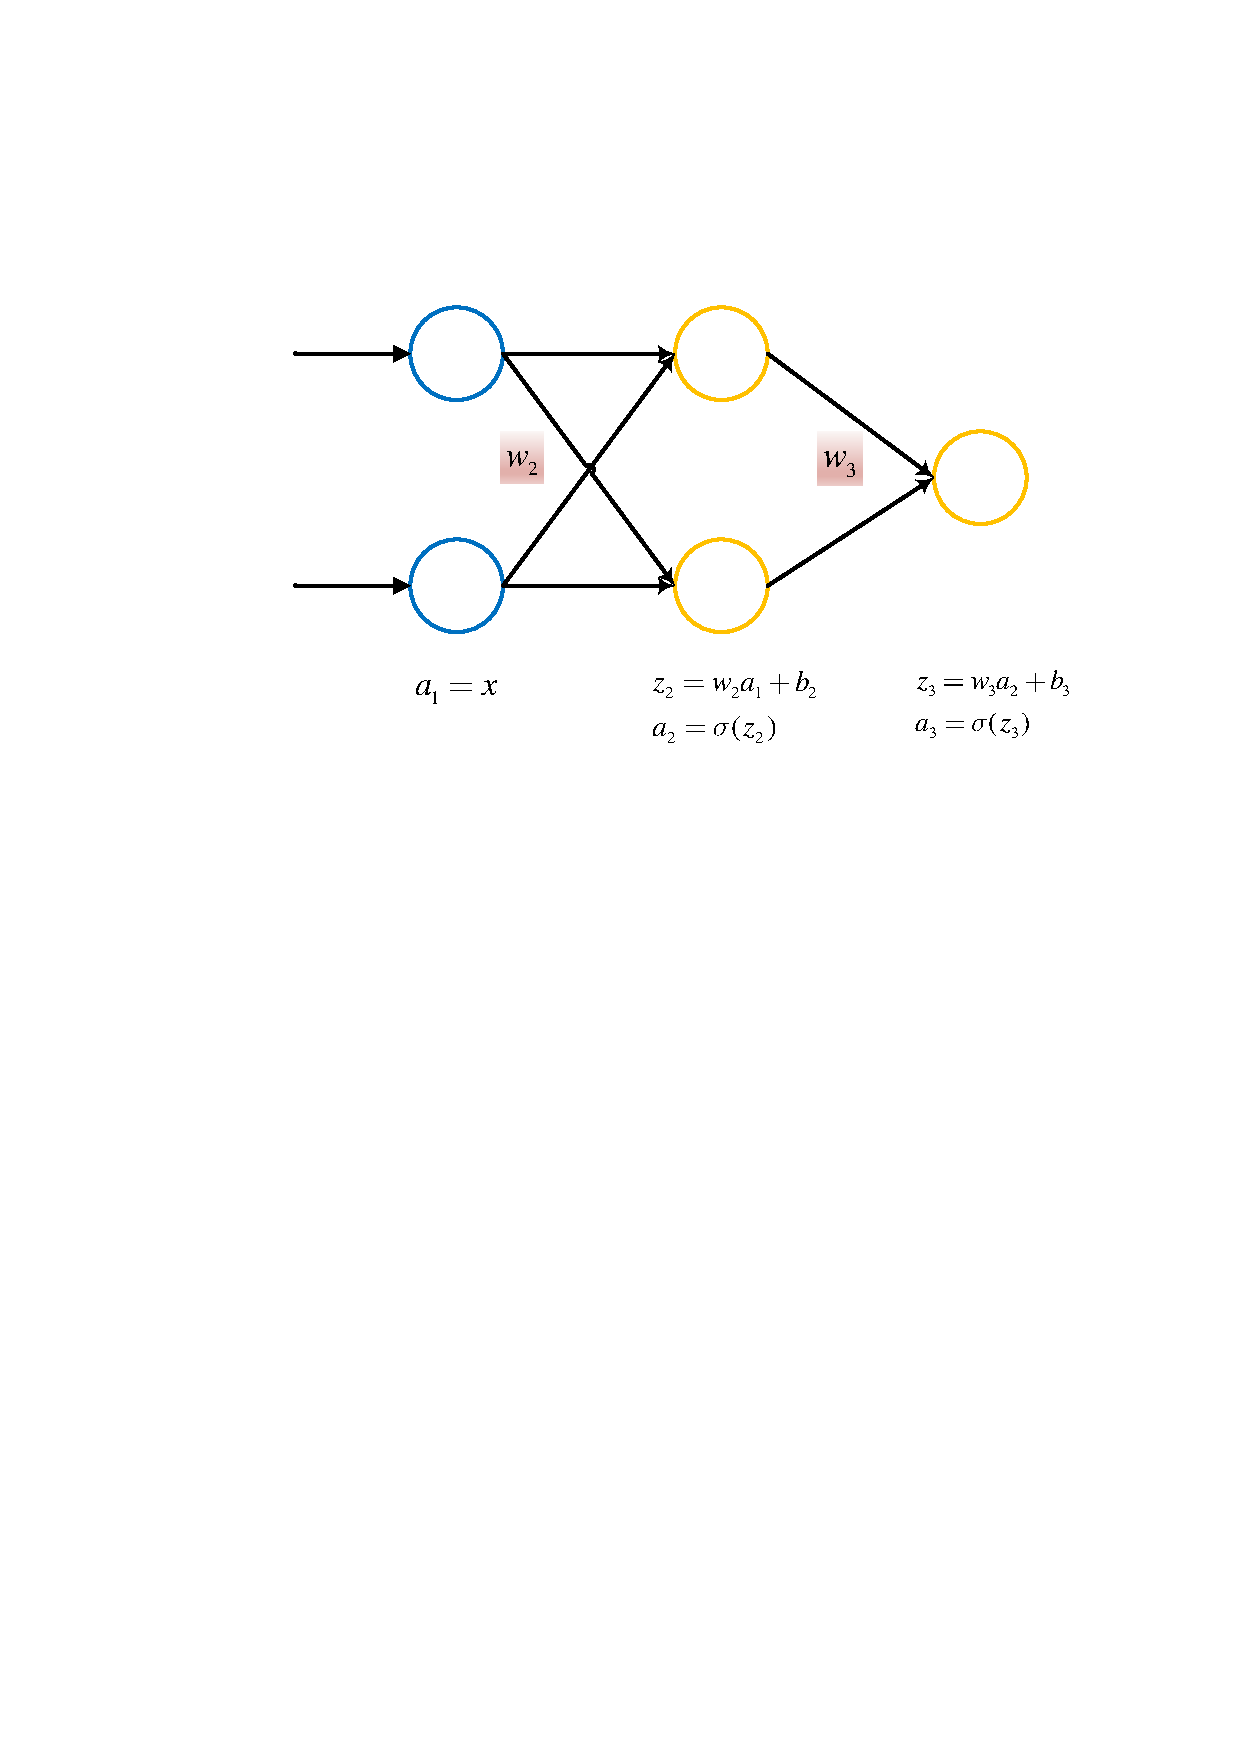
\includegraphics[width=8cm]{fig/Feedforward.pdf}
\caption{前向传播过程}
\end{figure}
\begin{lstlisting}
% Feedforward 前向传播计算成本函数
% w2大小 2 x 2
% w3大小 1 x 2
a1 = T'; 					% 输入层 a1大小 2 x 4
z2 = w2*a1+b2; 			% 第二层输入 z2大小 2 x 4
a2 = sigmoid(z2); 			% 第二层输出
z3 = w3*a2+b3;		% 第三层输入 z3大小 1 x 4
a3 = sigmoid(z3);			% 输出层 得到 1 x 4 的矩阵
cost = (a3-P').^2;
J(i) = sum(sum(cost, 2)) / m; 	% 求和得成本函数
\end{lstlisting}

\begin{figure}[H]
\centering
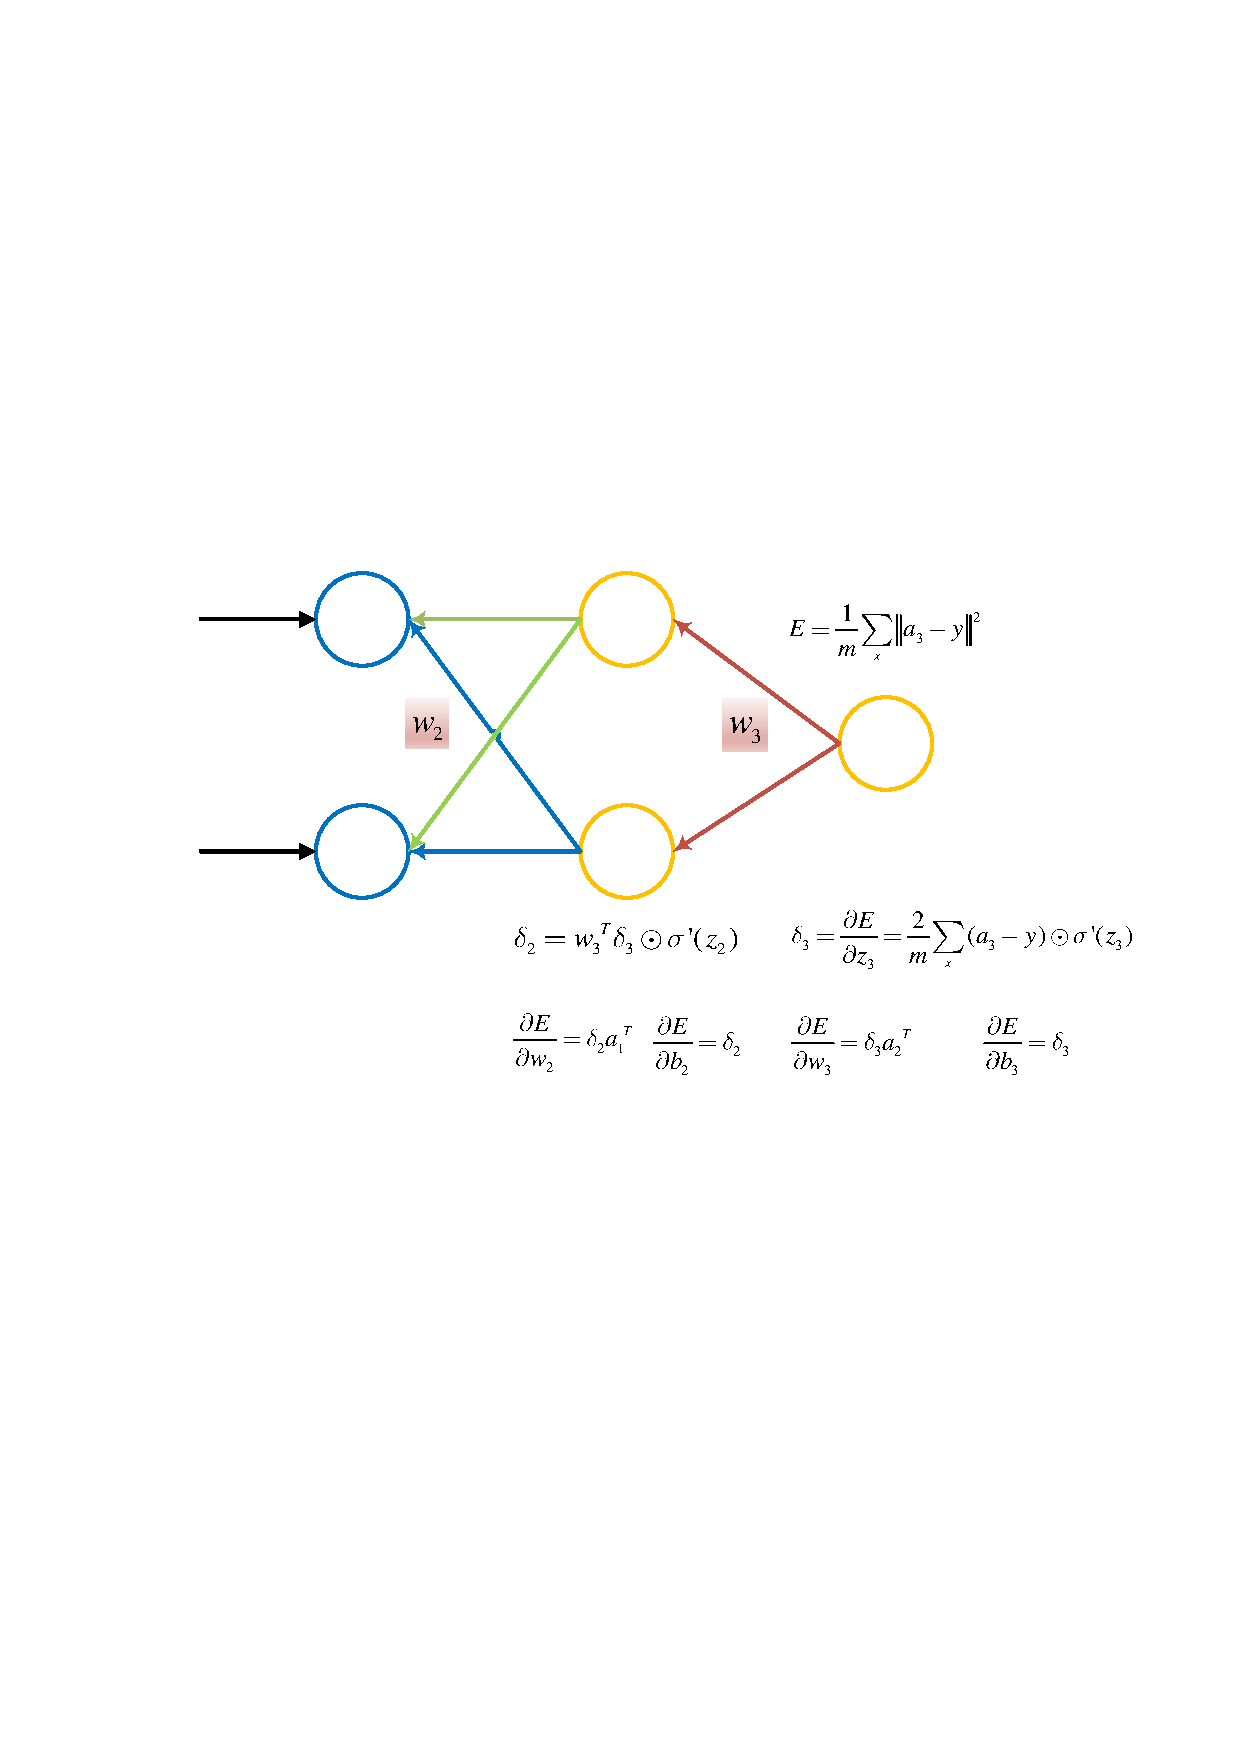
\includegraphics[width=13cm]{fig/Backpropagation.pdf}
\caption{反向传播过程}
\end{figure}

\begin{lstlisting}
% Backpropagation  反向传播计算梯度
Error3 =2/m*(a3-P').*d_sigmoid(z3); % 第三层的误差
Error2 = (w3)'*Error3.* d_sigmoid(z2);	% 第二层的误差

d_w3= Error3*a2'; % w2的梯度
d_b3= sum(Error3,2); % b3的梯度

d_w2= Error2*a1'; % w2的梯度
d_b2=sum(Error2,2); % b2的梯度
\end{lstlisting}


\begin{lstlisting}
%最后得到的各参数如下
w2 =
    5.6991    5.7146
    3.6140    3.6171

w3 =
    7.3065   -7.9139

b2 =
   -2.3530
   -5.5318

b3 =
   -3.2858

a3 =
    0.0640    0.9404    0.9404    0.0647

ans =
    0.0038
\end{lstlisting}

\begin{figure}[H]
\centering
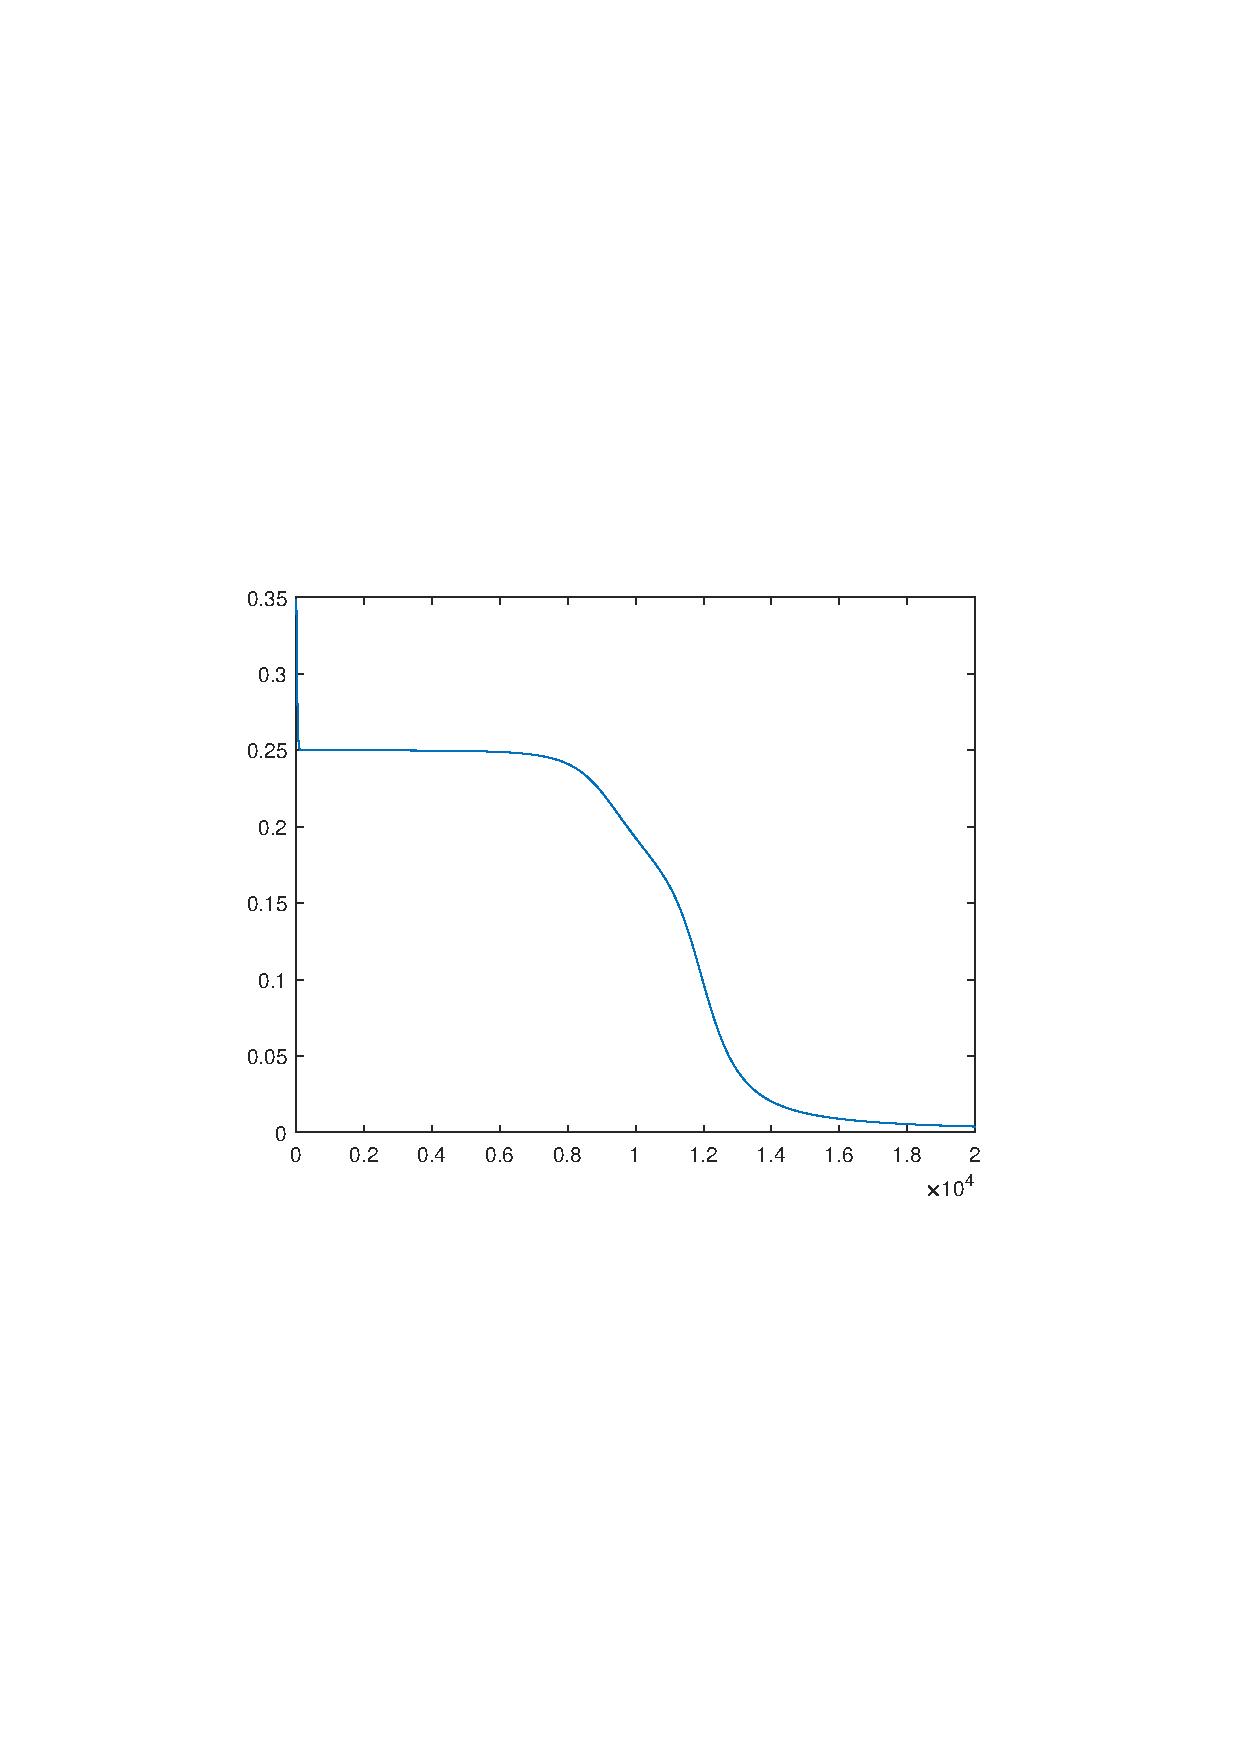
\includegraphics[width=10cm]{fig/xor1.pdf}
\caption{cost函数下降过程}
\end{figure}

观察图像我们可以发现:在刚开始迭代时,代价函数下降得非常快,但是在之后的前8000次迭代中,代价函数几乎没有下降,随后又突然急速下降,这是因为二次损失函数和Sigmoid激活函数组合时会发生\textbf{梯度消失}的现象.

下面我举一个简单的感知机例子来说明这种现象:
我们的输入为1,期望输出为0,将该感知机的权重和阈值初始化为0.6和0.9,那么第一次输出的结果为0.82,我们将学习速率定为$\eta=0.15$,迭代300次后停止,得到结果如下:
\begin{figure}[H]
\centering
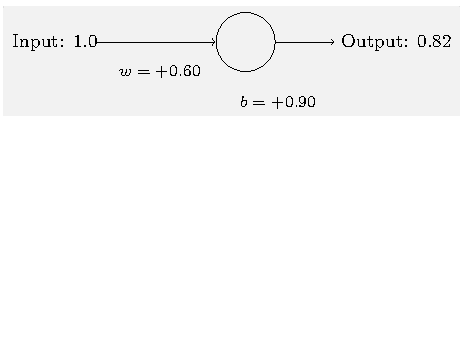
\includegraphics[width=8cm]{fig/1.pdf}
\caption{感知机}
\end{figure}

\begin{figure}[H]
\centering
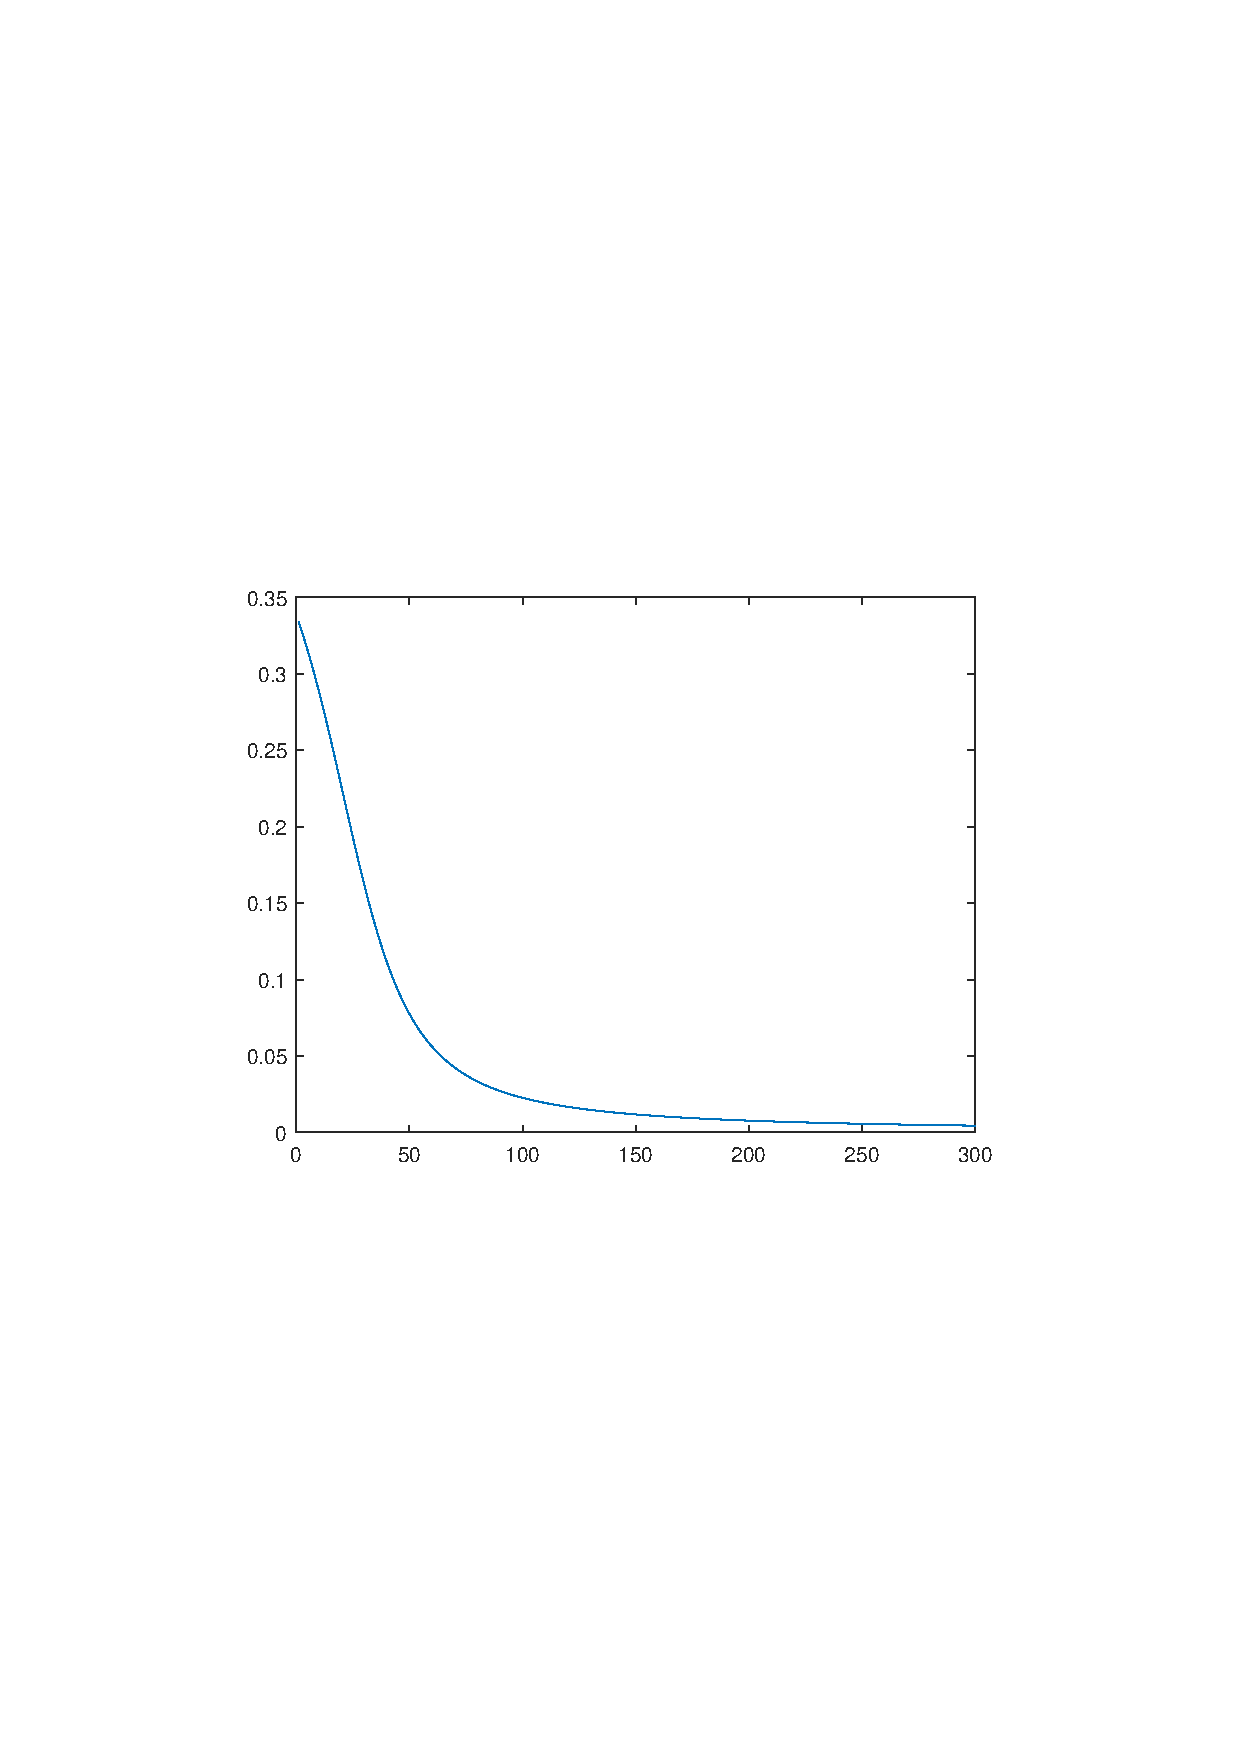
\includegraphics[width=7cm]{fig/test1.pdf}
\caption{初始化参数:$w=0.6,b=0.9$}
\end{figure}
这时我们看到感知机是像我们期望的那样快速收敛的,
但如果我们将感知机的权重和阈值初始化为2和2,
迭代结果却不一样了:

\begin{figure}[H]
\centering
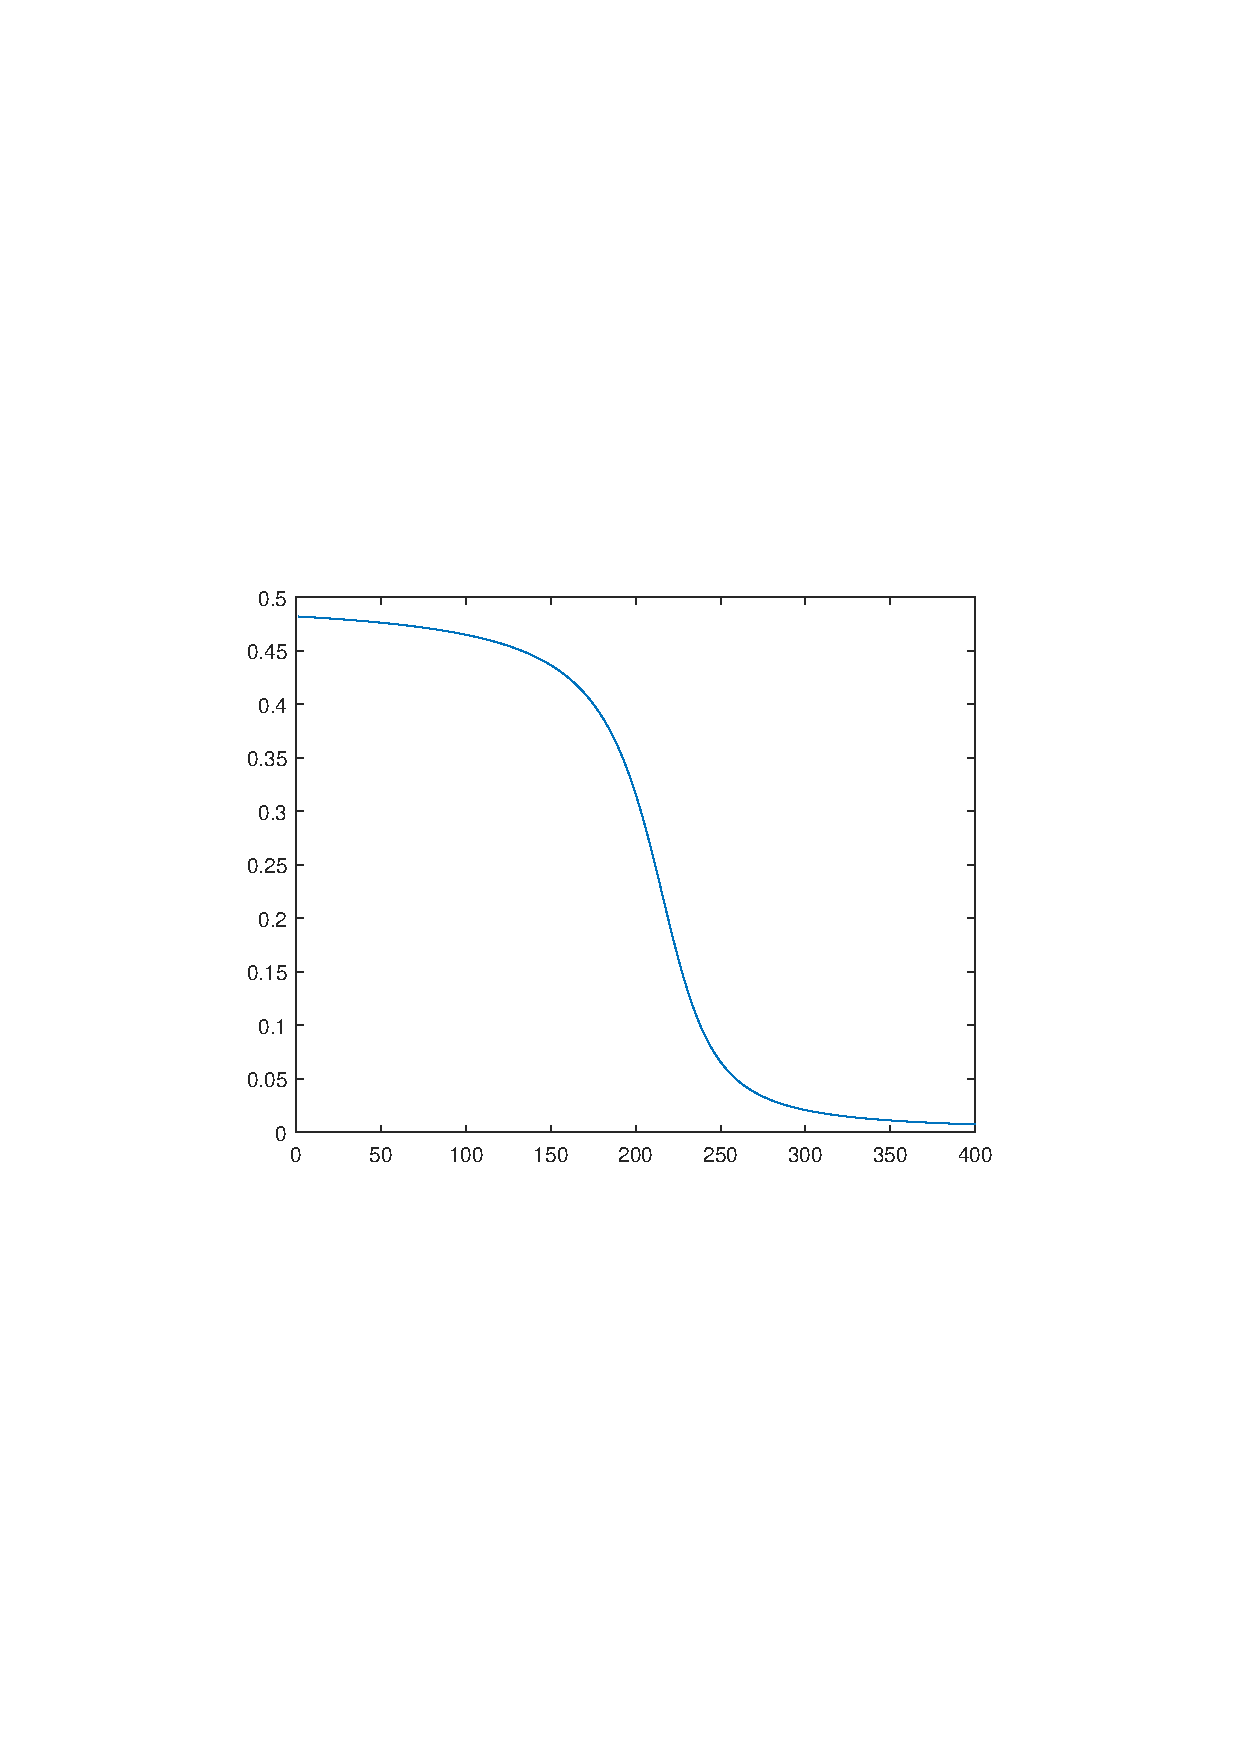
\includegraphics[width=7cm]{fig/test2.pdf}
\caption{初始化参数:$w=2,b=2$}
\end{figure}

图像呈现出来的结果也是先平缓下降,然后才加速,最后再减速。


\[E = \frac{1}{2}({a} - y)^2 \]
\begin{equation}
\frac{{\partial E}}{{\partial {w}}} = {a}\sigma'({z})x={a}\sigma'({z}) \label{dw1}
\end{equation}
\begin{equation}
\frac{{\partial E}}{{\partial {b}}} = a\sigma'({z}) \label{db1}
\end{equation}

\[\sigma'({z})=\sigma({z})(1-\sigma({z}))\]

从迭代公式中可以看出:当$\sigma({z})\rightarrow1\quad or\quad \sigma({z})\rightarrow0$时,$w,b$的梯度将会变得非常小,这会导致学习速率的缓慢,因此,我们可以将代价函数从二次函数替换为交叉熵函数,来改进神经网络。

\subsection{交叉熵代价函数}
定义代价函数为:
\[E = -y\ln a-(1-y)\ln (1-a) \]
那么可以求得:
\begin{equation}
\frac{{\partial E}}{{\partial {w}}} = (\sigma({z})-y)x \label{dw2}
\end{equation}
\begin{equation}
\frac{{\partial E}}{{\partial {b}}} = \sigma({z})-y \label{db2}
\end{equation}
对比等式(\ref{dw1})(\ref{dw2})可以发现:之前在二次代价函数里导致学习速率低的$\sigma'({z})$在等式(\ref{dw2})中刚好被消去了,并且这时学习速度也与误差$(\sigma({z})-y)$成正比了。

只要把原程序的$E,\partial E/\partial a_L$部分修改一下即可:
\begin{lstlisting}
cost = -P'.*log(a3)-(1-P').*log(1-a3);
J(i) = sum(sum(cost, 2)) / m; 	

Error3 =(a3-P')/m; 
\end{lstlisting}

交叉熵代价函数的下降过程如下:

\begin{figure}[H]
\centering
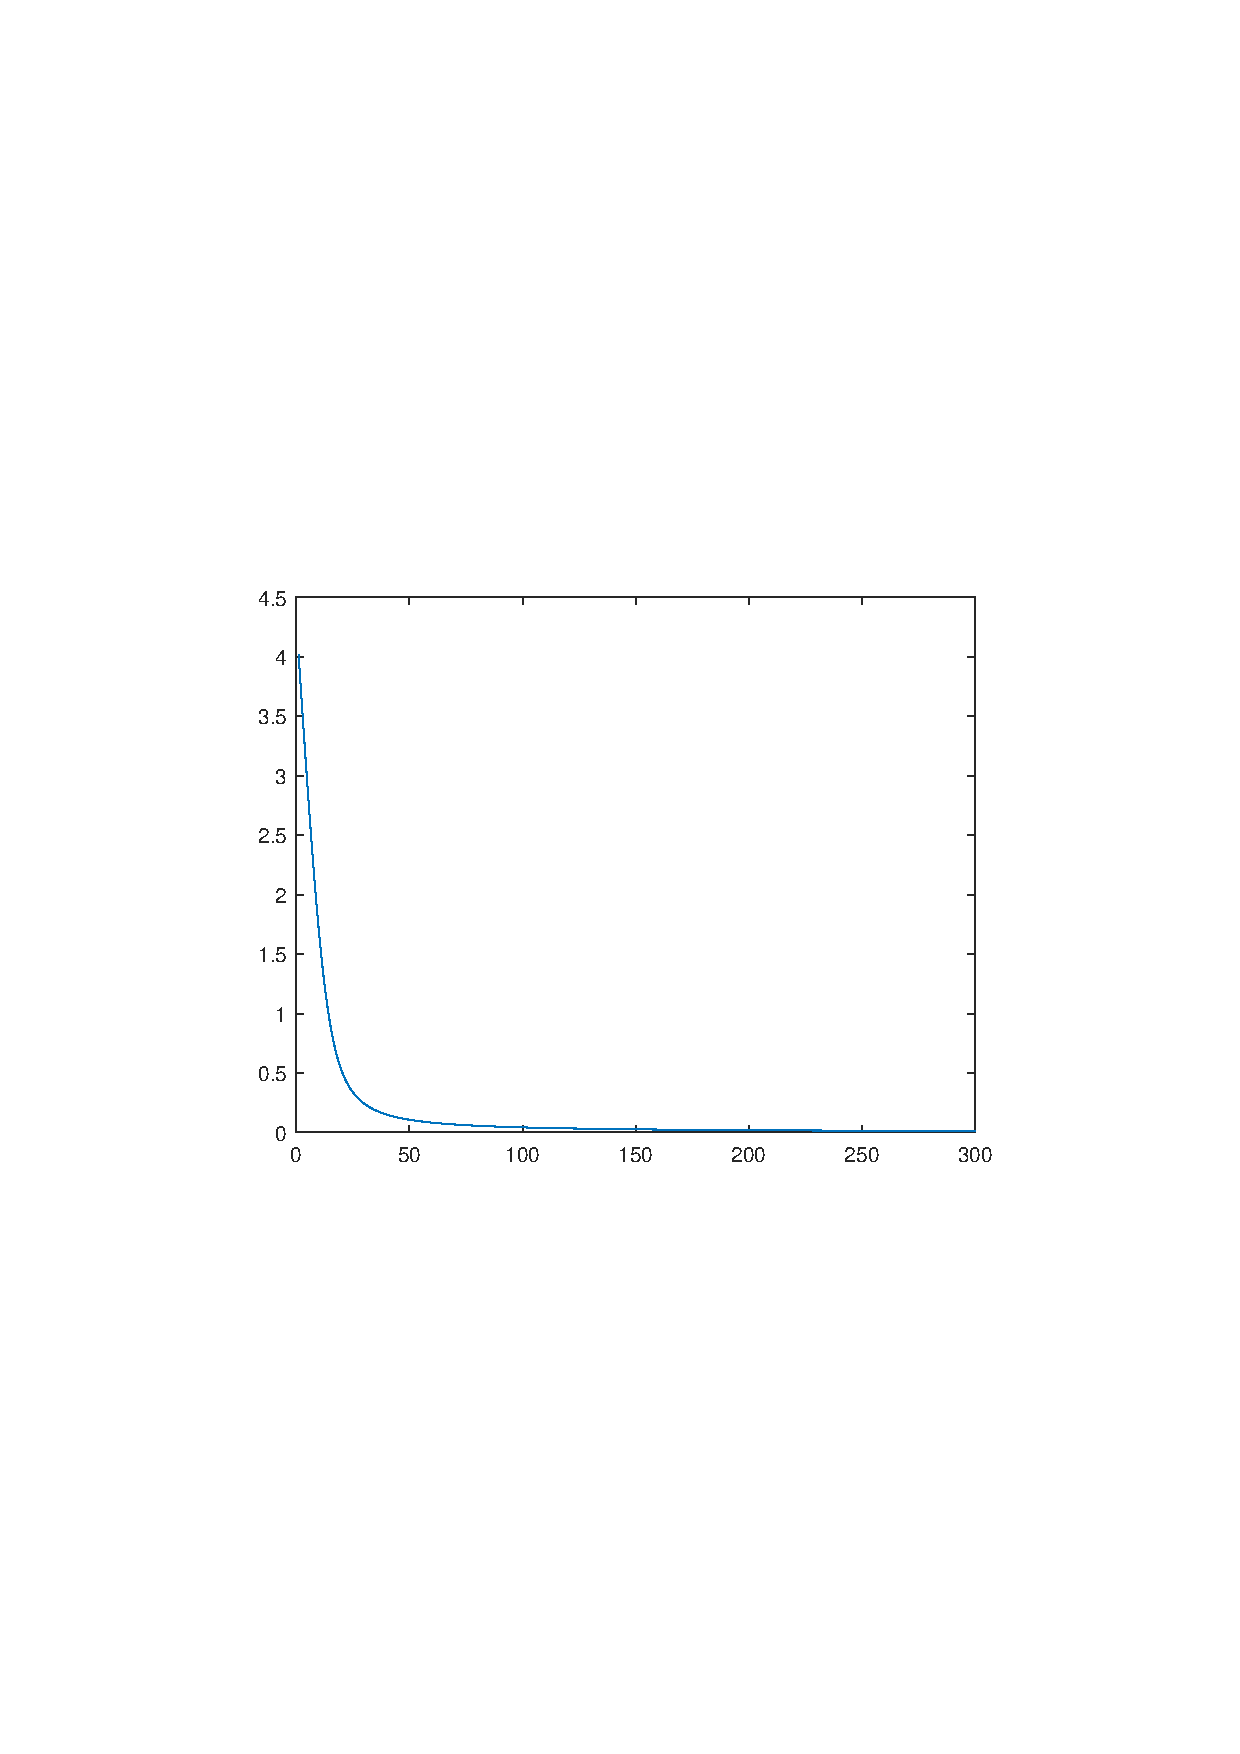
\includegraphics[width=8cm]{fig/test3.pdf}
\caption{交叉熵感知机程序}
\end{figure}

我们也能使用交叉熵代价函数来改造我们原来的xor程序,运行结果如下:
\begin{figure}[H]
\centering
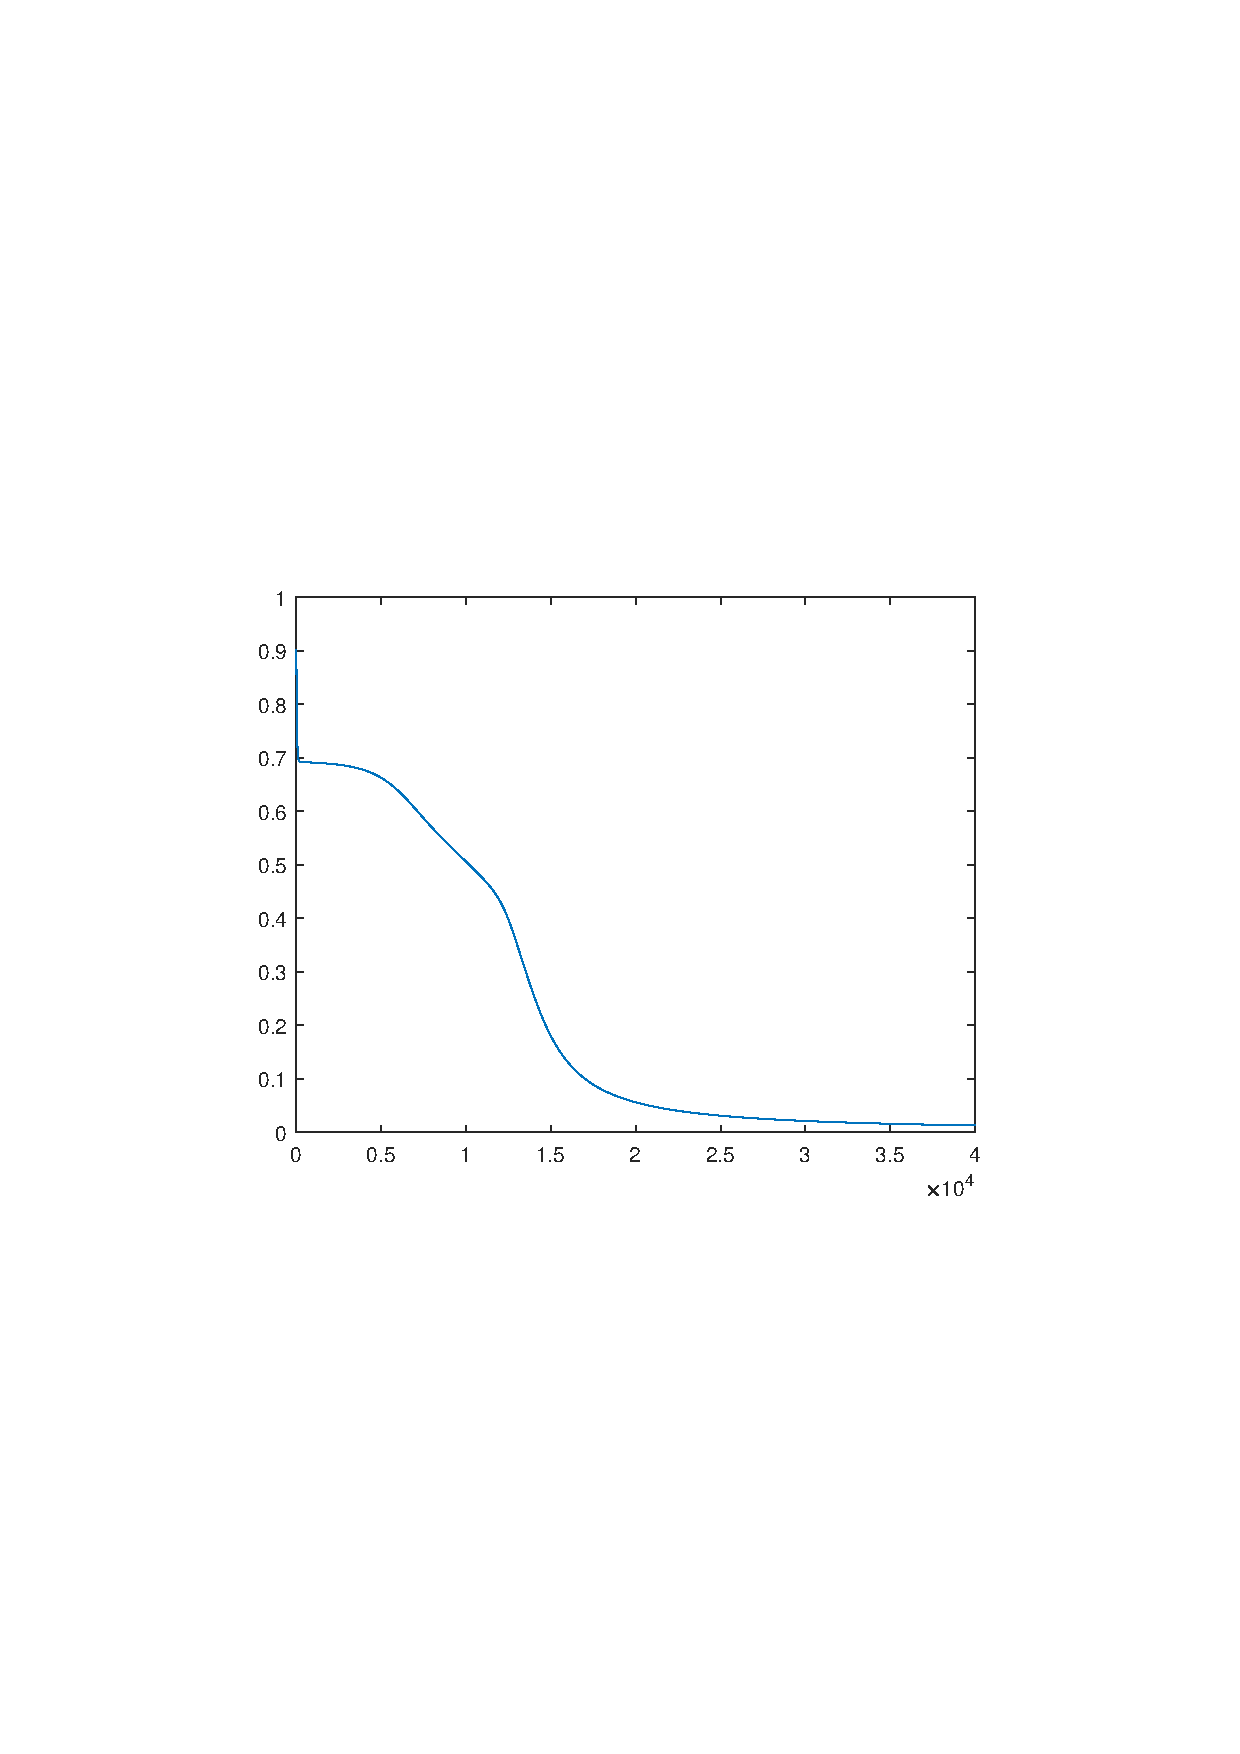
\includegraphics[width=8cm]{fig/xor2.pdf}
\caption{交叉熵xor程序}
\end{figure}
\newpage
\begin{lstlisting}
w2 =
    4.7028    4.6939
    6.8040    6.7488

w3 =
  -10.9213   10.1324

b2 =
   -7.1907
   -3.0075

b3 =
   -4.6355

a3 =
    0.0153    0.9883    0.9882    0.0129

ans =
    0.0130
\end{lstlisting}

\subsection{动量项momentum}
动量项是将梯度下降更新规则 $w\rightarrow w'=w-\eta\nabla E$ 改成
\begin{align} 
  v \rightarrow v' &= \mu v - \eta \nabla E \\
  w \rightarrow w' &= w+v' 
\end{align}


如果梯度在上一次迭代的方向和这一次的方向相同,那么,改变量就会叠加,
朝那个方向移动的速度就会增加,
而如果方向不同,那么则会抵消一部分,使得反方向运动的速度慢下来。
这个与物体运动中的惯性有些类似,因此称为动量项。

添加了动量项的xor程序运行结果如下:
\begin{lstlisting}
w2 =
    7.3616    7.3609
    5.4367    5.4366

w3 =
   12.3830  -13.2183

b2 =
   -3.3630
   -8.3198

b3 =
   -5.7669

a3 =
    0.0047    0.9966    0.9966    0.0035
    
ans =
    0.0037
\end{lstlisting}

\begin{figure}[H]
\centering
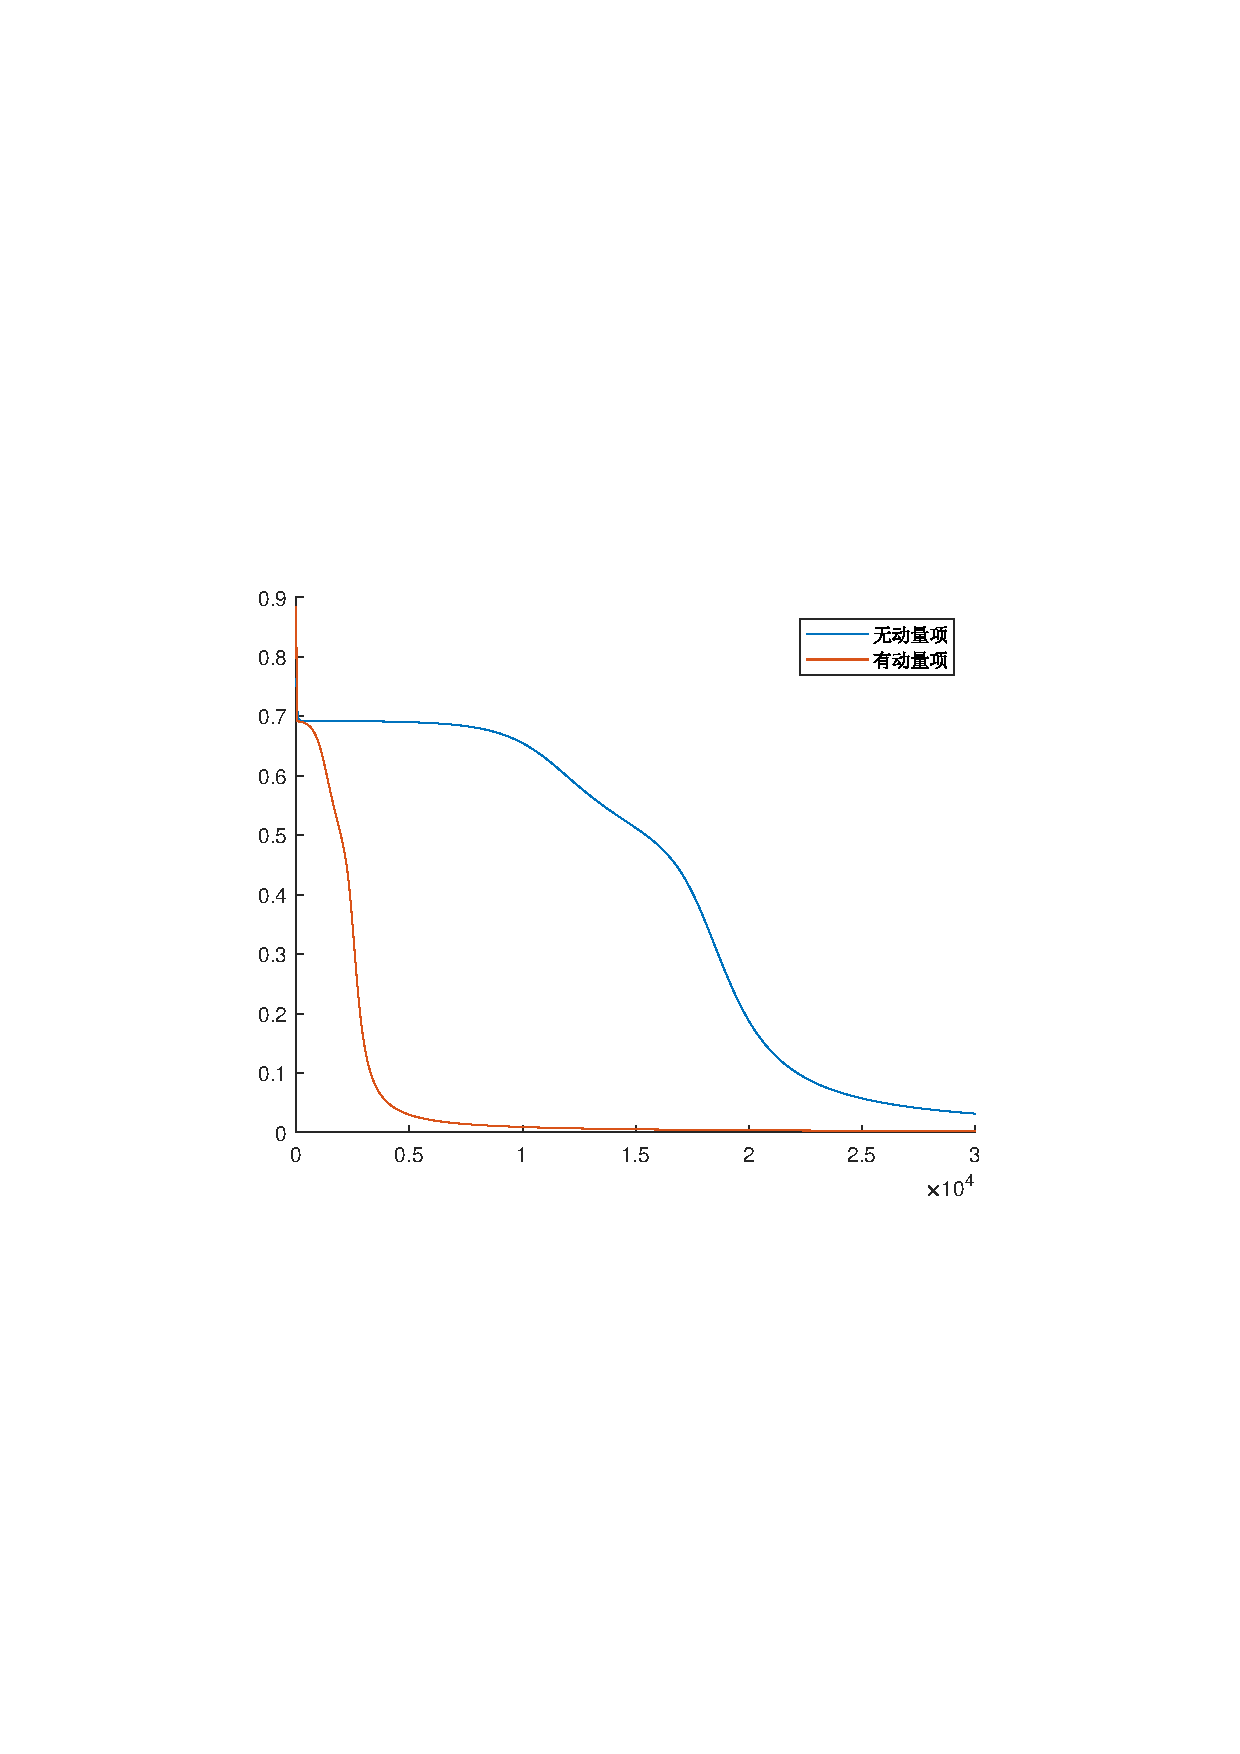
\includegraphics[width=10cm]{fig/compare.pdf}
\caption{对比}
\end{figure}

可以明显地看出,添加了动量项后,神经网络收敛的速度有了非常大的提升。
\newpage
\section{奇偶判别问题}
对于一串长度为$N$的二进制输入,判断串中1的个数是否为奇数,解决此类问题的神经网络通常构架为:$[N,N,1]$,即$N$个输入单元,$N$个隐藏单元,1个输出单元。

下面以$N=4$为例来解决这个问题。

首先是生成数据:将从0到$2^N-1$的数字转化为二进制,储存为输入向量T,然后生成对应的期望输出P.

\begin{lstlisting}
N=4;
T = abs(dec2bin(0:(2^N-1), N))-48;
P=mod(sum(T, 2),2);
save data2.mat T P
\end{lstlisting}

然后将之前编好之前的三层神经网络程序模板稍微改动一下,可得到运行结果如下:

\begin{figure}[H]
\centering
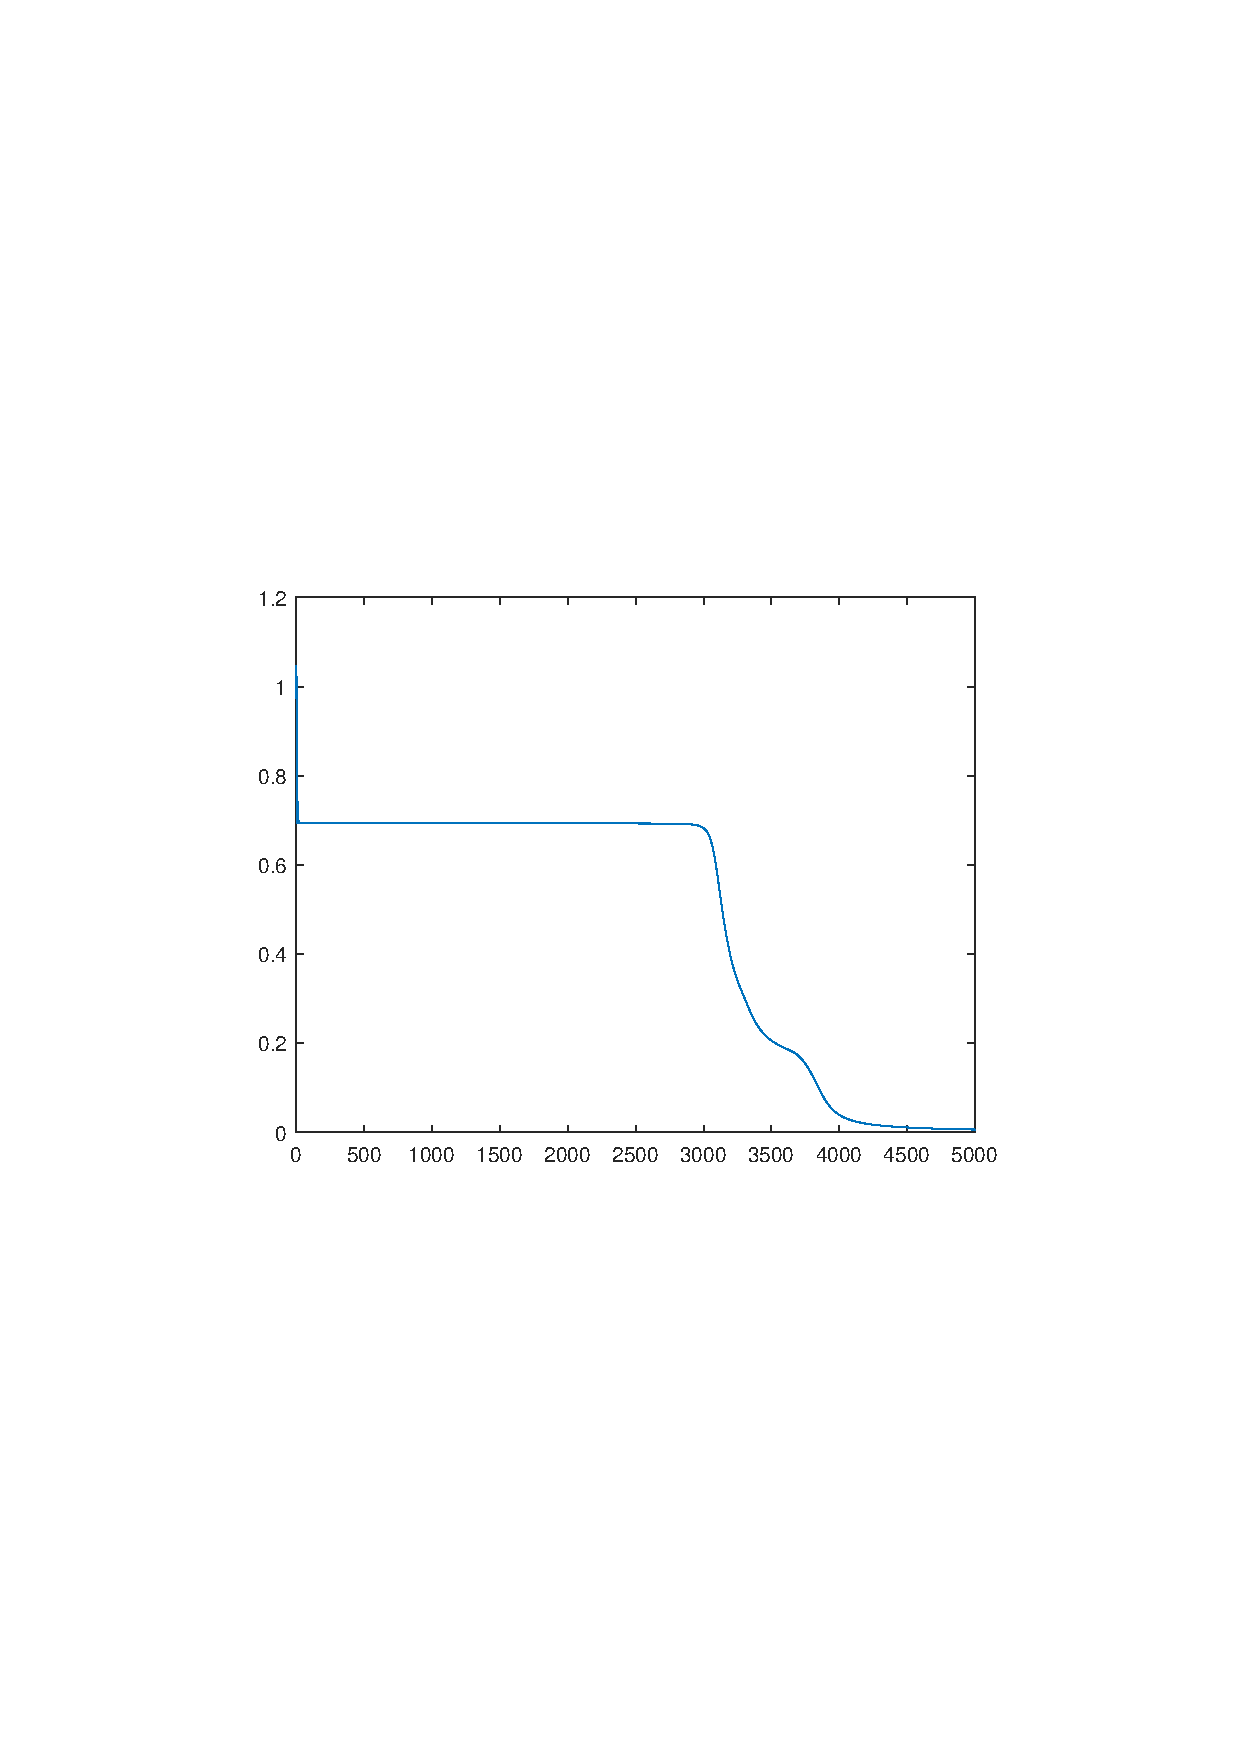
\includegraphics[width=10cm]{fig/parity.pdf}
\caption{cost函数下降过程}
\end{figure}

\newpage
\begin{lstlisting}
w2 =
    5.6930    5.6926    5.6940   -5.4309
    4.0606    4.0606    4.0606   -4.8899
    6.4270    6.4271    6.4268   -6.9895
    7.7000    7.7003    7.6988   -7.9590

w3 =
  -12.8905   14.3991  -14.9507   14.5050

b2 =
    2.7115
  -10.2916
   -9.1962
   -3.5978

b3 =
    5.7940

a3 =
  1 至 4 列
    0.0027    0.9933    0.9982    0.0021
  5 至 8 列
    0.9982    0.0021    0.0034    0.9986
  9 至 12 列
    0.9982    0.0021    0.0034    0.9986
  13 至 16 列
    0.0034    0.9986    0.9931    0.0020

ans =
    0.0028
\end{lstlisting}

仔细观察神经网络的权值,可以发现一个特点:$w_2$每一行的左边三列都是近似相等的,而最右边一列则近似为它们的相反数,并且每一行的绝对值相差都不大,在$w_3$中,则表现为正负号交替,且绝对值也相差不大,这与作者给出的样例类似\footnote{样例中为正负1交替},这验证了作者的观点:这这样的网络模型中,由学习规则所创建的内部表示将会使得被激活的隐藏神经元的数量等于输入中的“1”的数量,由$w_3$中正负号交替的性质,当有奇数个隐藏神经元被激活时,输出为1,偶数个隐藏神经元被激活时,输出为0.输出层的神经元能否被激活只依赖于激活隐藏神经元的数量,而不在于哪个输入神经元是否被激活,这正是奇偶性所要求的编码。

\newpage
\section{编码问题}
\textbf{编码问题}:将一组正交input pattern映射到一组正交output pattern.
\subsection{编码问题1}
\begin{table}[!tbh]
\caption{\quad 编码问题1}
\centering
\begin{tabular}{c c c}  \hline
\qquad 输入\,\,\,\,\,\,\,\,\,\,\,\, &	&\qquad 输出\,\,\,\,\,\,\,\,\,\,\,\, \\ \hline
10000000&$\rightarrow$&10000000\\
01000000&$\rightarrow$&01000000\\
00100000&$\rightarrow$&00010000\\
00010000&$\rightarrow$&00010000\\
00001000&$\rightarrow$&00001000\\
00000100&$\rightarrow$&00000100\\
00000010&$\rightarrow$&00000010\\
00000001&$\rightarrow$&00000001\\\hline
\end{tabular}
\label{Tcode1}
\end{table}

这一类编码问题的构架为$[N,\log_2N,N]$,在这种情况下,我们要通过隐藏神经元(hidden units)给每个N位的input pattern编码,将其映射到$\log_2N$位的二进制模式,然后再将其解码至N位的output pattern.
\begin{lstlisting}
a3 =
0.9797    0.0000    0.0000    0.0003    0.0000    0.0083    0.0069    0.0115
0.0000    0.9659    0.0370    0.0000    0.0005    0.0000    0.0058    0.0009
0.0000    0.0224    0.9421    0.0322    0.0024    0.0000    0.0000    0.0000
0.0000    0.0000    0.0209    0.9446    0.0000    0.0209    0.0000    0.0071
0.0000    0.0042    0.0105    0.0001    0.9777    0.0151    0.0005    0.0000
0.0095    0.0000    0.0000    0.0169    0.0111    0.9666    0.0000    0.0000
0.0206    0.0345    0.0000    0.0000    0.0001    0.0000    0.9567    0.0046
0.0040    0.0022    0.0016    0.0078    0.0000    0.0000    0.0000    0.9876

ans =
    0.0761
\end{lstlisting}

\begin{figure}[H]
\centering
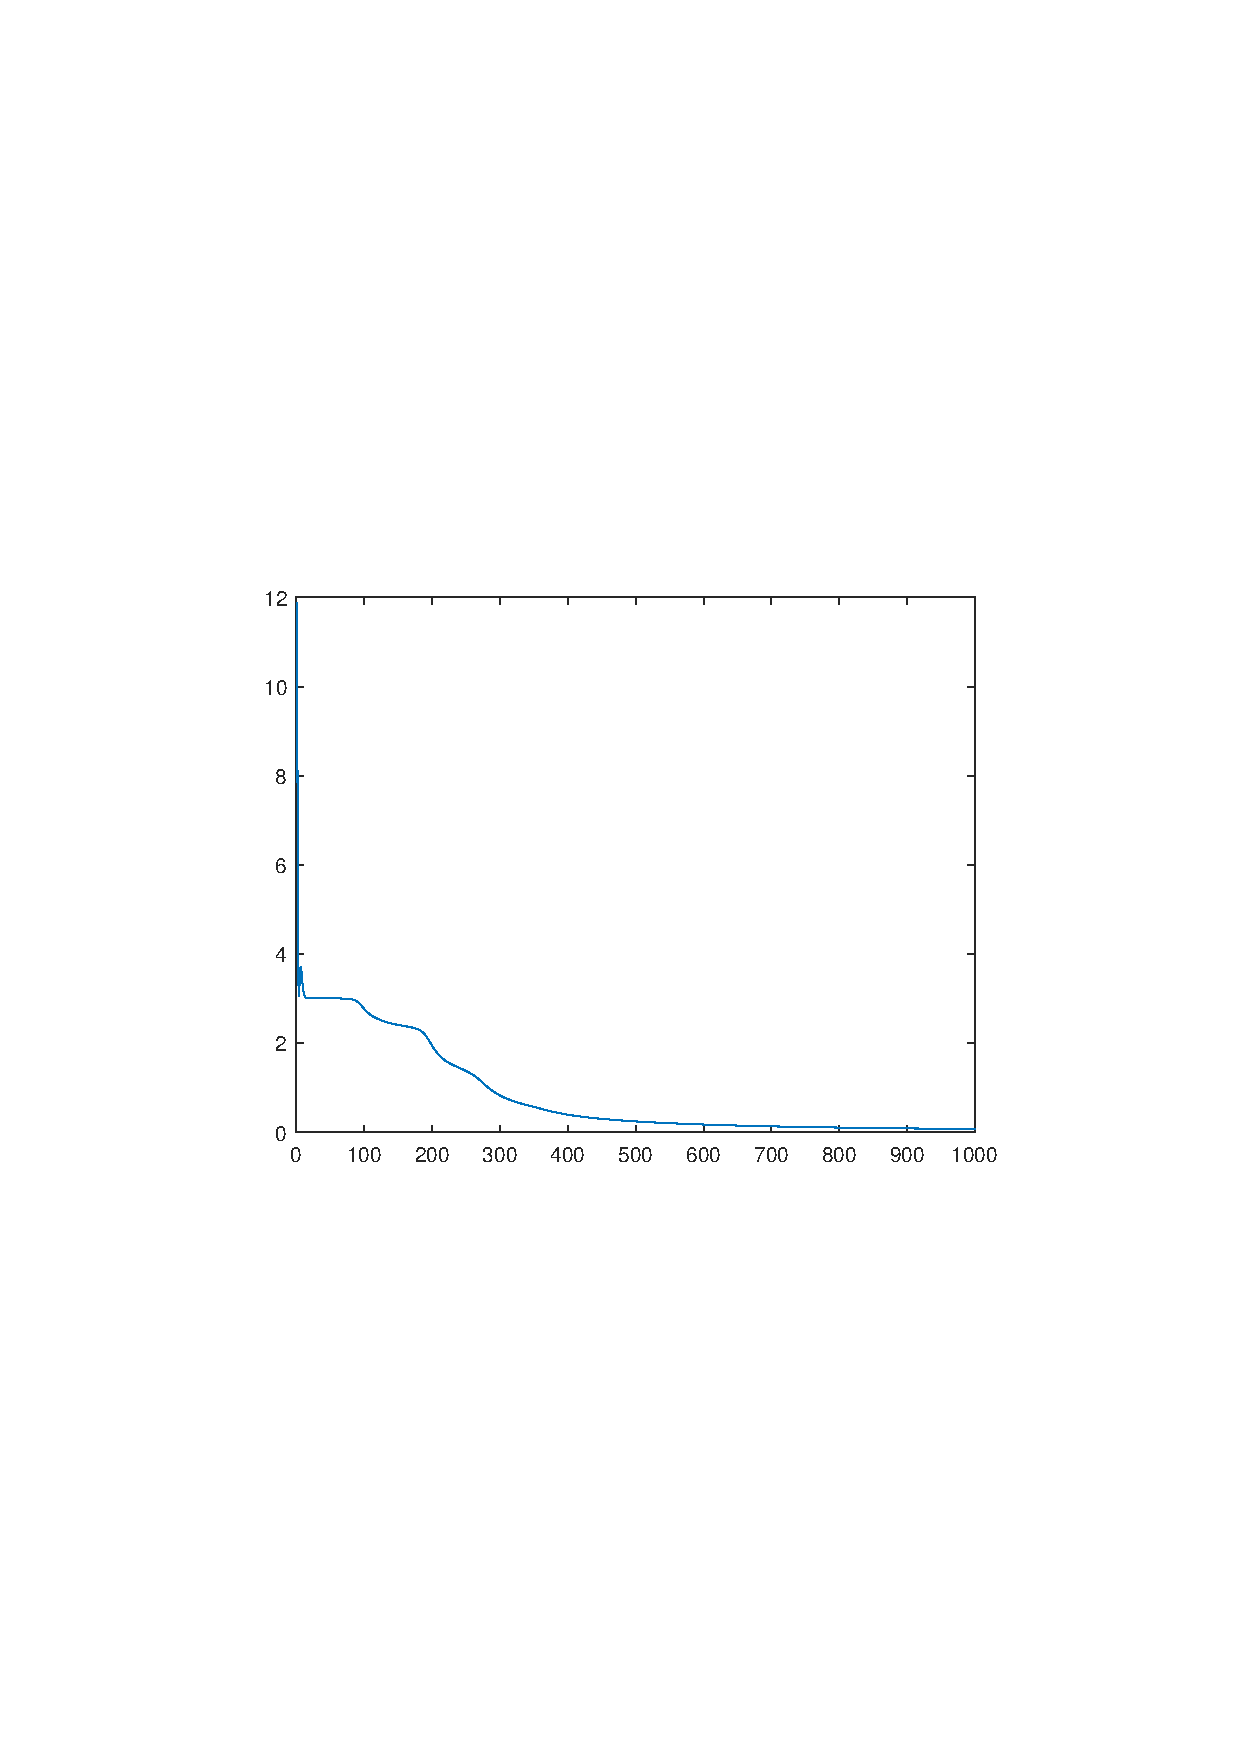
\includegraphics[width=10cm]{fig/encode1.pdf}
\caption{cost函数下降过程}
\end{figure}

\subsection{编码问题2}
\begin{table}[!tbh]
\caption{\quad 编码问题2}
\centering
\begin{tabular}{c c c}  \hline
\qquad 输入\,\,\,\,\,\,\,\,\,\,\,\, &	&\qquad 输出\,\,\,\,\,\,\,\,\,\,\,\, \\ \hline
00&$\rightarrow$&1000\\
01&$\rightarrow$&0100\\
10&$\rightarrow$&0010\\
11&$\rightarrow$&0001\\\hline
\end{tabular}
\label{Tcode24}
\end{table}

该类编码问题中,我们要把两单元的分散式表示转化成四单元的局部表示,离散输入模式的相似性结构将不会被保留到局部输出表示中。为了解决这个问题,系统首先要把输入模式的分散式表示转化成不同的激活值,对应于不同输入模式下单一隐藏神经元的中间值,然后将其转化到另一个分散式表示,最后转换为局部表示。(注意:此处的分散式表示Distributed Representation指一个个体用几个编码单元而不是一个编码单元表示,即一个个体分布在几个编码单元上)。

因此此题中要求的构架为$[2,1,4,4]$,不能继续套用之前的三层神经网络模板了,于是我用结构体编写了一个N层神经网络的模板,因为MATLAB中的三维矩阵不能储存维数不一致的矩阵,所以只好用结构数组,代码更直观的同时,速度却慢了很多。

\begin{lstlisting}
L(num_layers).a =
    0.9859    0.0067    0.0000    0.0068
    0.0068    0.9940    0.0000    0.0000
    0.0000    0.0000    0.9950    0.0045
    0.0105    0.0000    0.0108    0.9824

ans =
    0.0224
\end{lstlisting}

\begin{figure}[H]
\centering
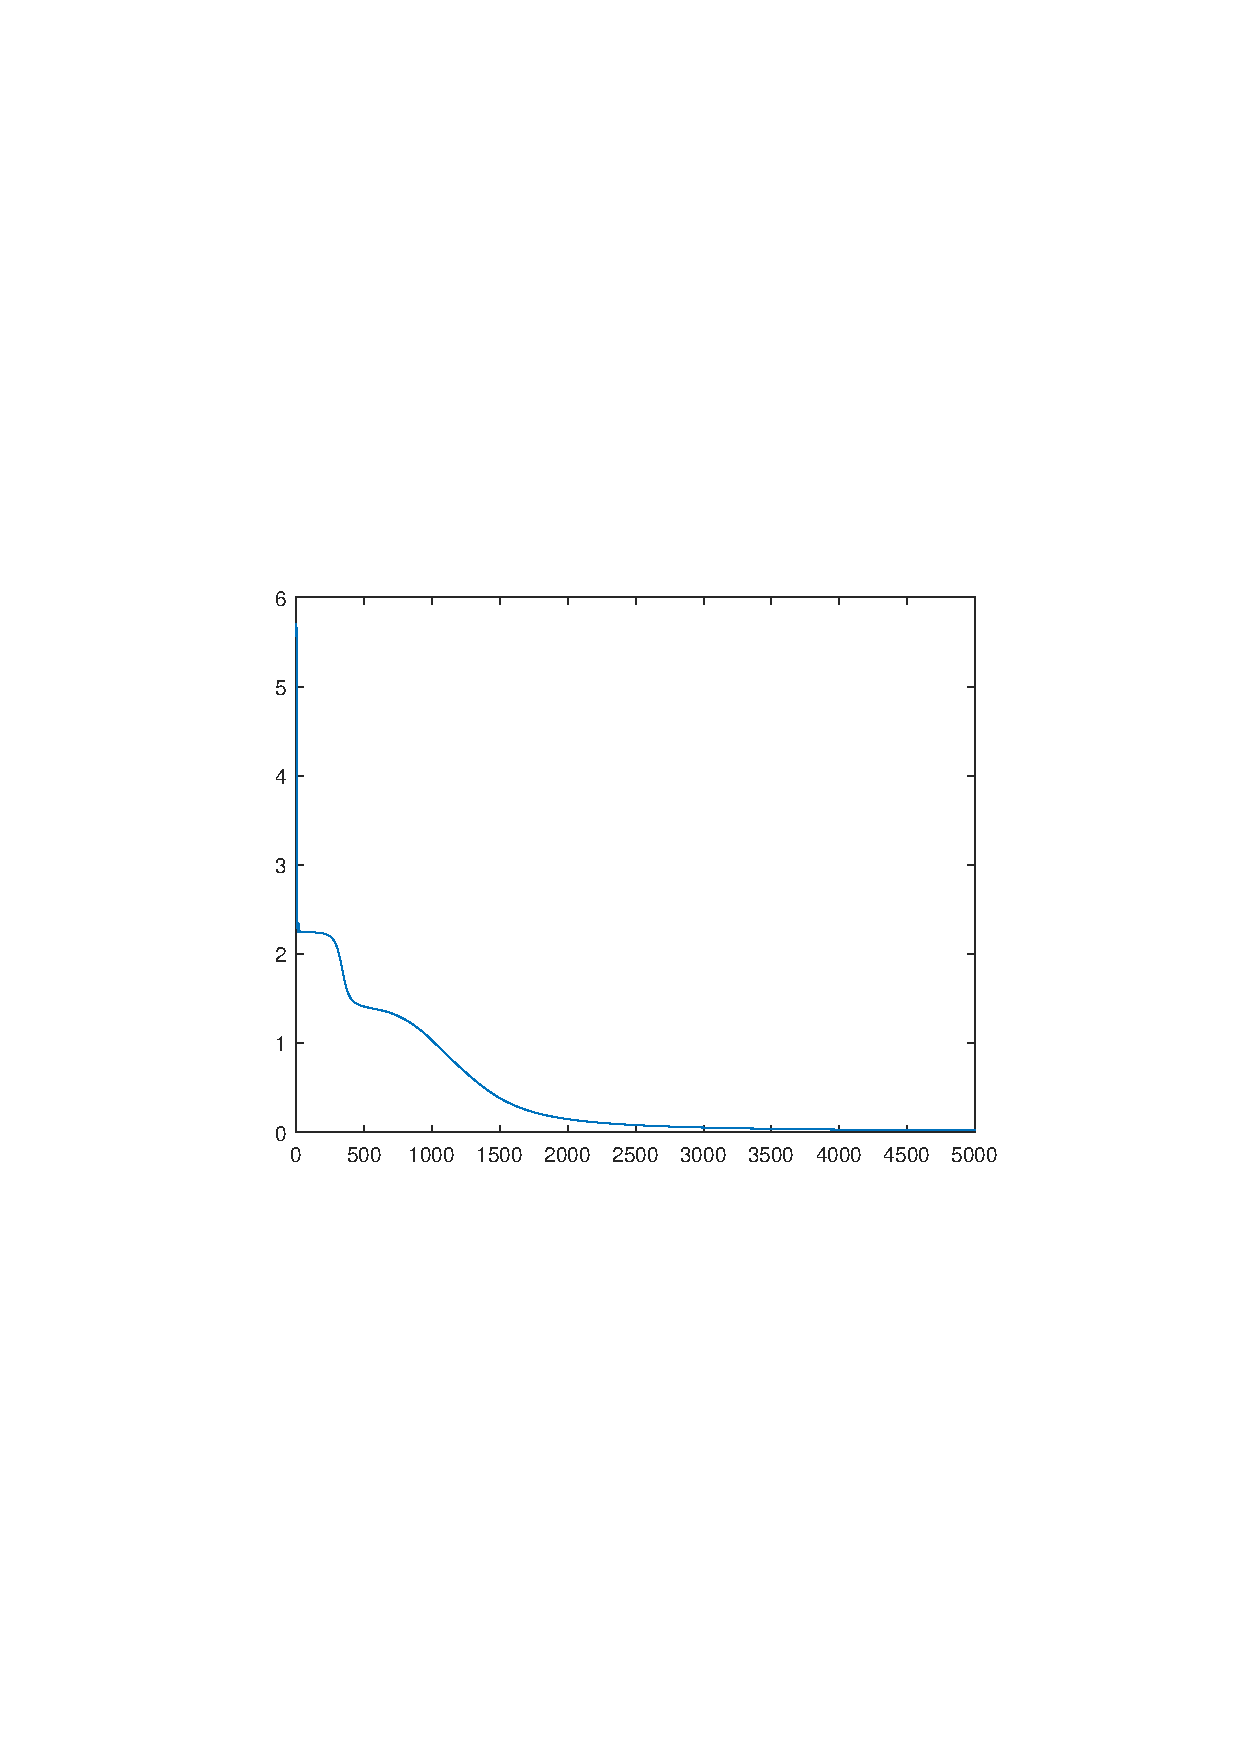
\includegraphics[width=10cm]{fig/encode2.pdf}
\caption{cost函数下降过程}
\end{figure}

\newpage
\section{对称问题}
\textbf{对称问题:}对于一串二进制输入,判断是否是中心对称的.

\begin{figure}[H]
\centering
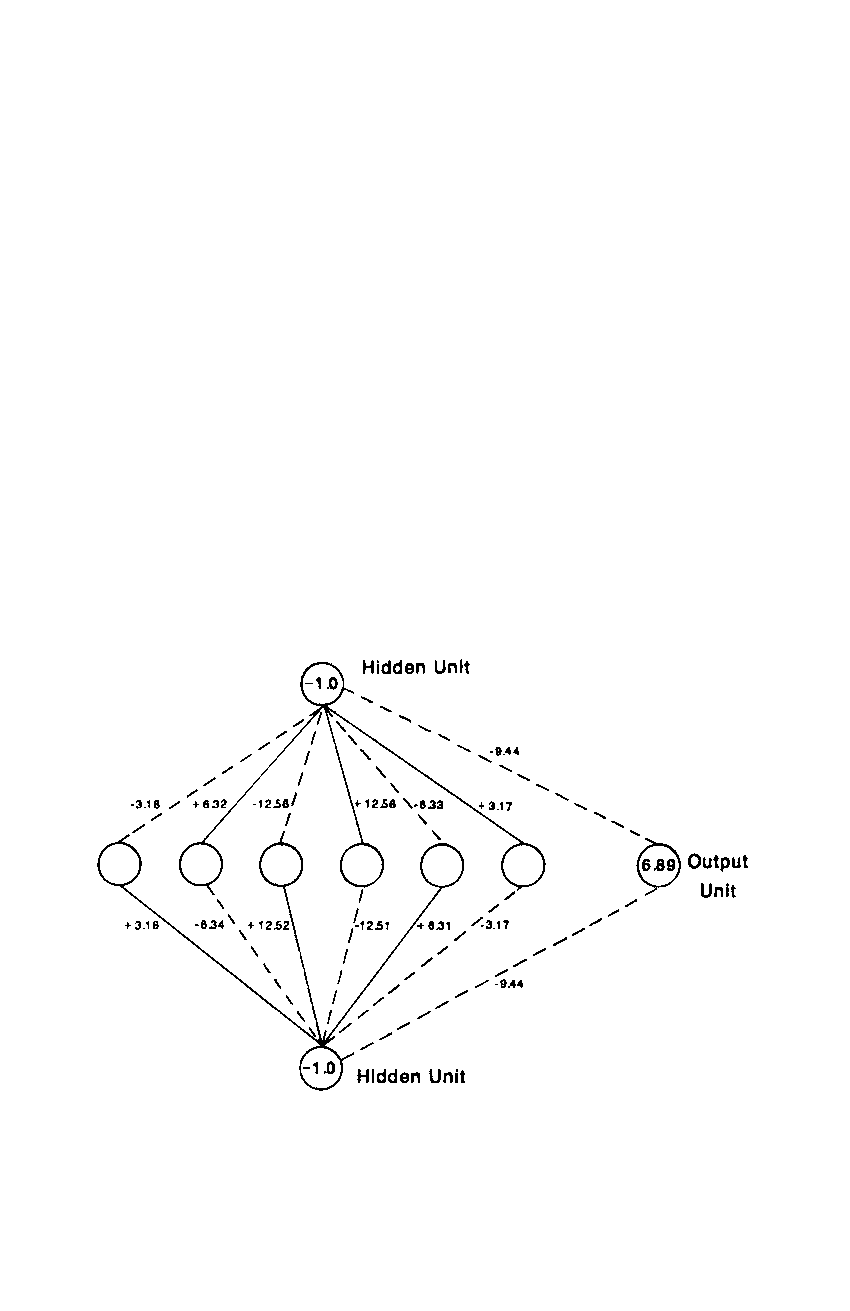
\includegraphics[width=10cm]{fig/symmetry0.pdf}
\caption{一个解决对称问题的网络结构}
\end{figure}
从例子中可以看出:由于权值关于上下左右的对称性,当输入并非对称时,上下两个hidden units至少有一个会被激活,从而导致输出神经元被关闭。

此外,书中还指出:每条边的权值之比为1:2:4,这使得右边三个神经元发送到隐藏层的总激活值唯一,使得左侧的非对称输入难以精确平衡抵消掉。最后,只有当两个hidden units都处于未激活状态时,输出神经元才会被激活。

将学习速率调为1后,得到了很好的输出结果如下:

观察输出的$w_2,w_3$,每条边的权值之比确实精确为1:2:4,权值、偏置也具有对称性,很好地吻合了Hinton的结论.
\begin{lstlisting}
L(2).w =
    3.6554    7.2908   14.5102  -14.5128   -7.2938   -3.6593
   -3.4807   -6.9357  -13.7993   13.7964    6.9322    3.4746

L(3).w =
  -19.3936  -19.6933

L(2).b =
   -2.4196
   -2.3128

L(3).b =
    8.7942
   
ans =
   2.0560e-04
\end{lstlisting}

\begin{figure}[H]
\centering
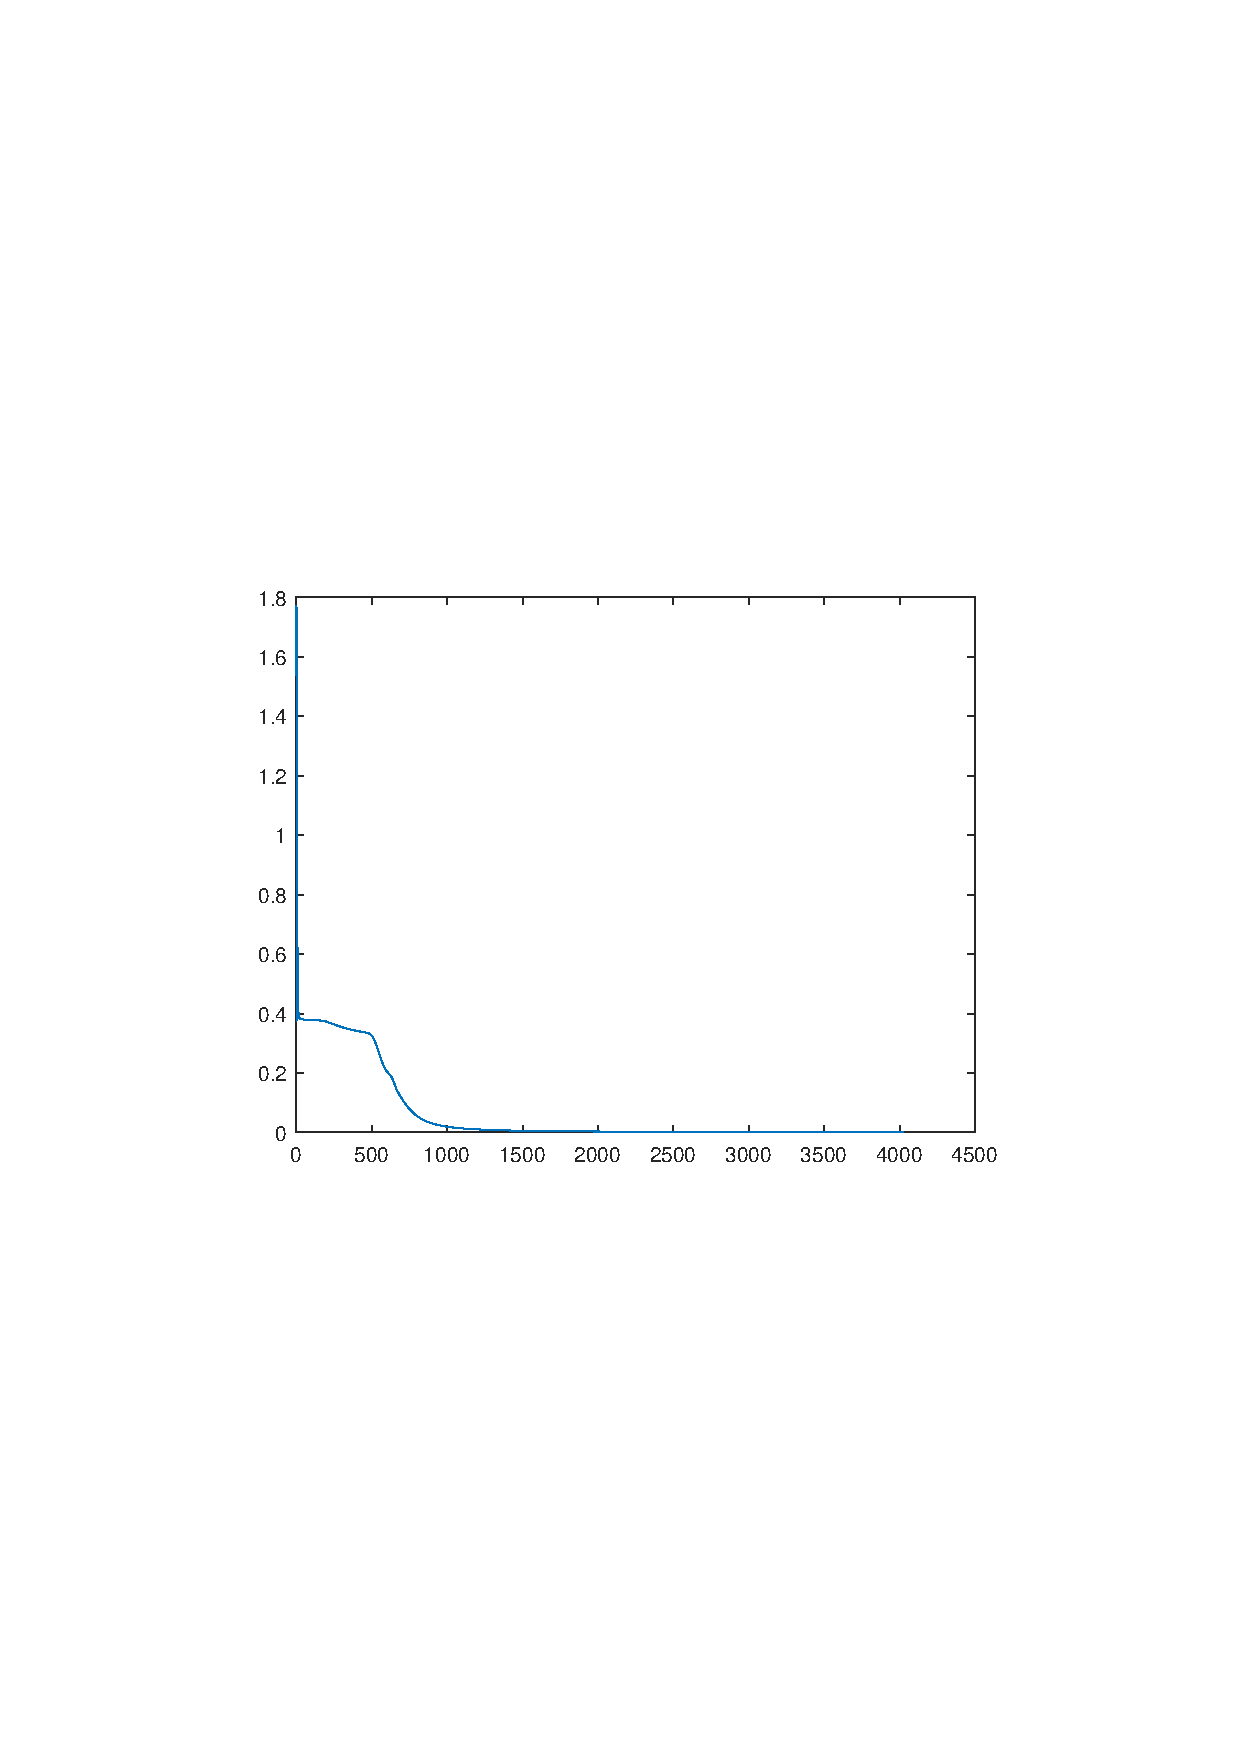
\includegraphics[width=7cm]{fig/symmetry1.pdf}
\caption{cost函数下降过程}
\end{figure}

此外,在调试程序的过程中,还添加了minibatch法,取minibatch的size=40,也得到了不错的输出:
\begin{figure}[H]
\centering
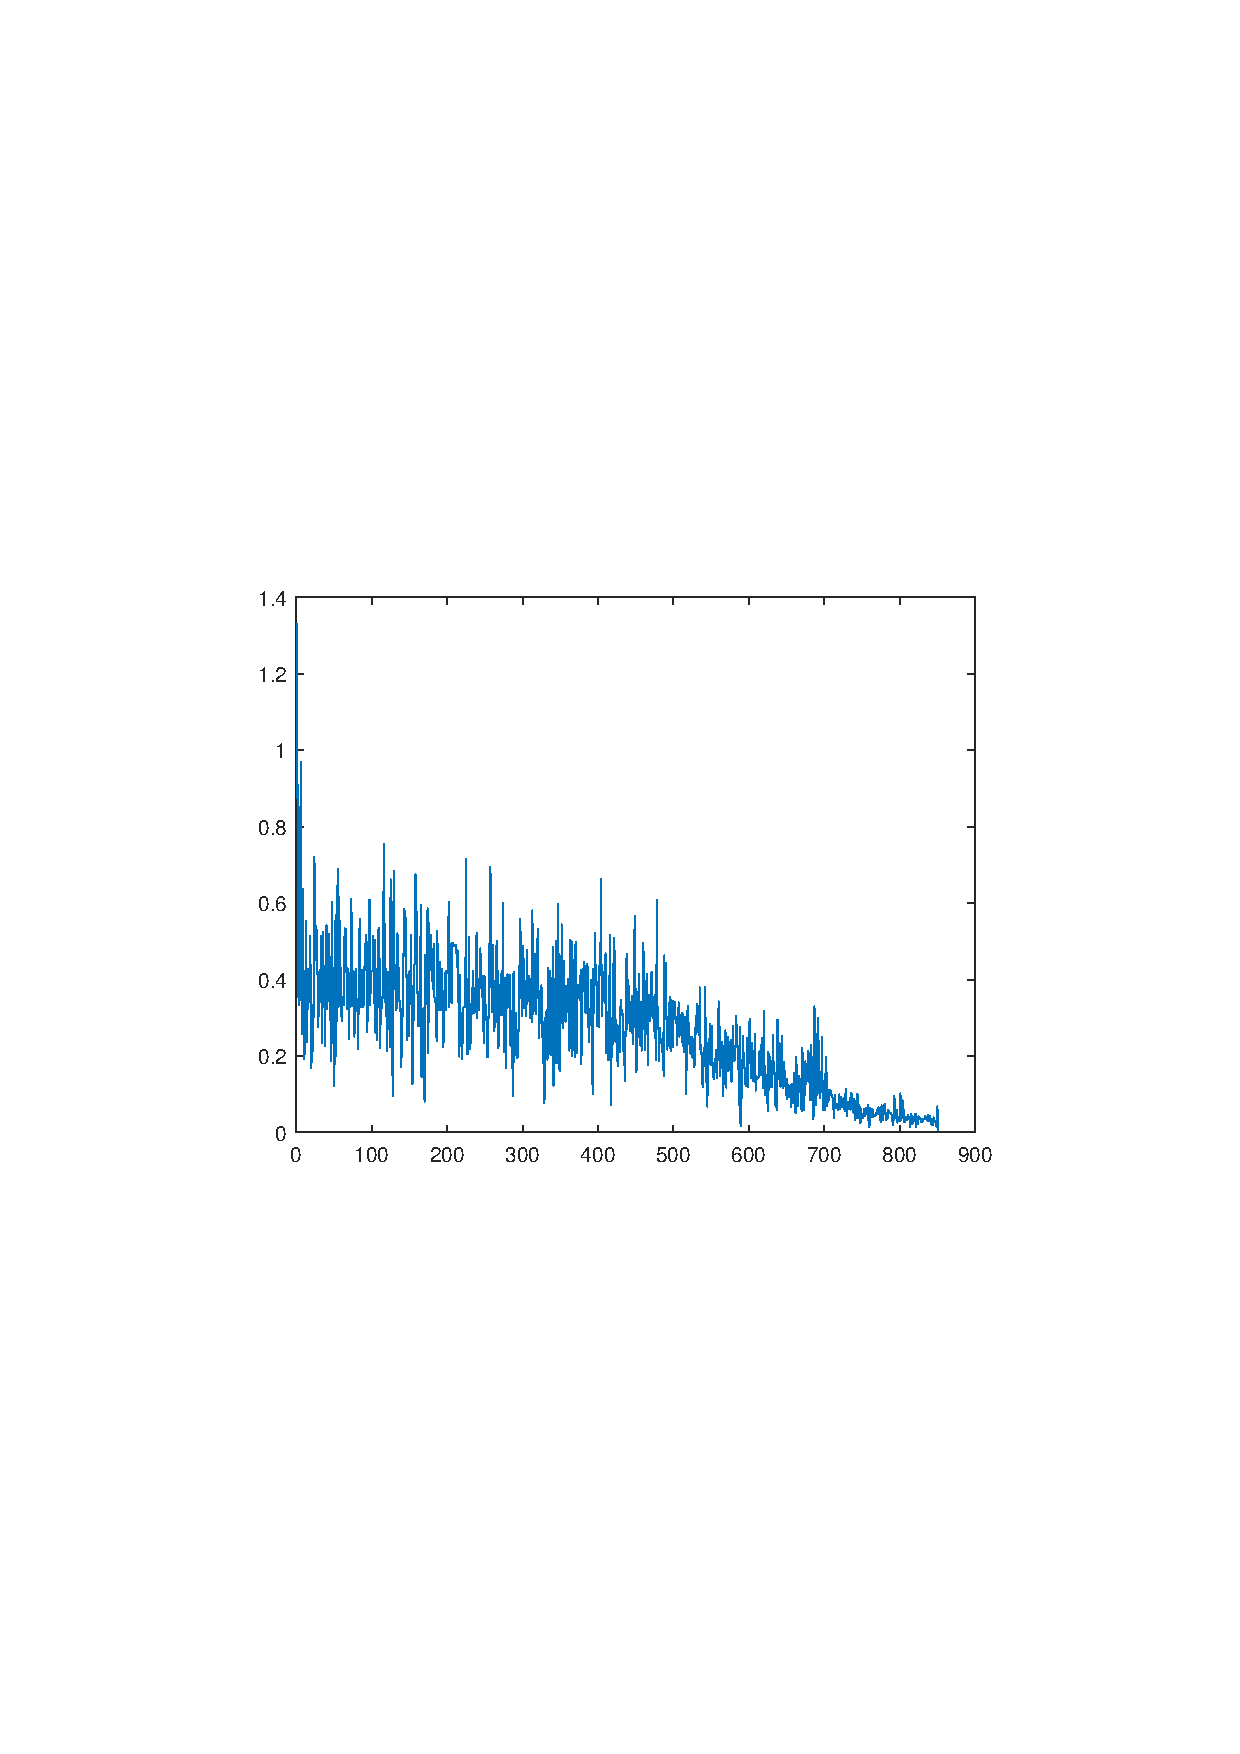
\includegraphics[width=7cm]{fig/symmetry2.pdf}
\caption{minibatch法}
\end{figure}

\end{document}